%% The following is a directive for TeXShop to indicate the main file
%%!TEX root = diss.tex
\chapter{Supporting Materials}

% This would be any supporting material not central to the dissertation.
% For example:
% \begin{itemize}
% \item radiometry
% \item technical details of MVS, PS, SL, SfS, etc
% \end{itemize}

\section{Definition of 3D Reconstruction}
\label{sec:3DRecon_Def}
We will first provide definitions of some basic concepts, which include general computer vision concepts such as scene, camera, and image. We then define a few other terms that are closely related to the reconstruction problem. We then provide reasonable approximations for a more practical definition of the problem as a whole.

\subsection{Basic notations}
We will use the following notations: $\{C_n\}_{n=0}^{N-1}$ represents the camera set, which includes both intrinsic and extrinsic parameters; $\{I_n\}_{n=0}^{N-1}$ represents the set of all images; $\{L_n\}_{n=0}^{N-1}$ represents the set of light sources.

\noindent\textbf{Definition 1 (Scene)} The scene $S$ is the four-dimensional joint spatio-temporal target of interest.

\noindent\textbf{Definition 2 (Image)} The image refers to the 2D observation of the 3D scene $S$ on the image plane of camera $C_i$ at time $t_0$, which is modelled as: $I_i = T(S, C_i, L_0, t_0)$, or on the image plane of $C_0$  under the light source $L_i$ at time $t_i$, $I_i= T(S, C_0, L_i, t_i)$, where $T$ is the geometric/radiometric transformation.

$T$ can be a geometric transformation which determines the 2D coordinates of a 3D point, or a radiometric transformation which determines the intensity/irradiance information from the information of illumination, viewing direction and surface orientation.

\subsection{Segment and Scell}
\noindent\textbf{Definition 3 (Segment)} A segment ($seg$) is a distinct region in the image, and is the most basic element in the image, which can be considered as a generalized pixel. 

For instance, a segment can be a pixel, a window area, an edge, a contour, or a region of arbitrary size and shape.

\noindent\textbf{Definition 4 (Cue)} Cues are the visual or geometric characteristics of the segments $seg$ that can be used for reconstruction, denoted as $cue(seg)$.

For instance, the cue can be the texture within a window area, the intensity/colour value of a pixel, or the object contour, etc.

\noindent\textbf{Definition 5 (Scell)} A scell (scene element, denoted as $sc$) is a volume in the scene which corresponds to at least one segment. A scell can be considered as a generalization of a voxel.
 % However, a scell is not necessarily distinct since

\noindent\textbf{Definition 6 (Property)} Properties are the visual and geometric characteristics of the scell $sc$, which would influence the cues of a segment, denoted as $prop(sc)$.

The property of the scell can be the 3D position or orientation information, visual texture, reflectance, surface orientation, roughness, convacity, etc.

The relation between the terms defined above is shown in Figure~\ref{fig:scell_seg}.
\begin{figure}[!htbp]
\centering
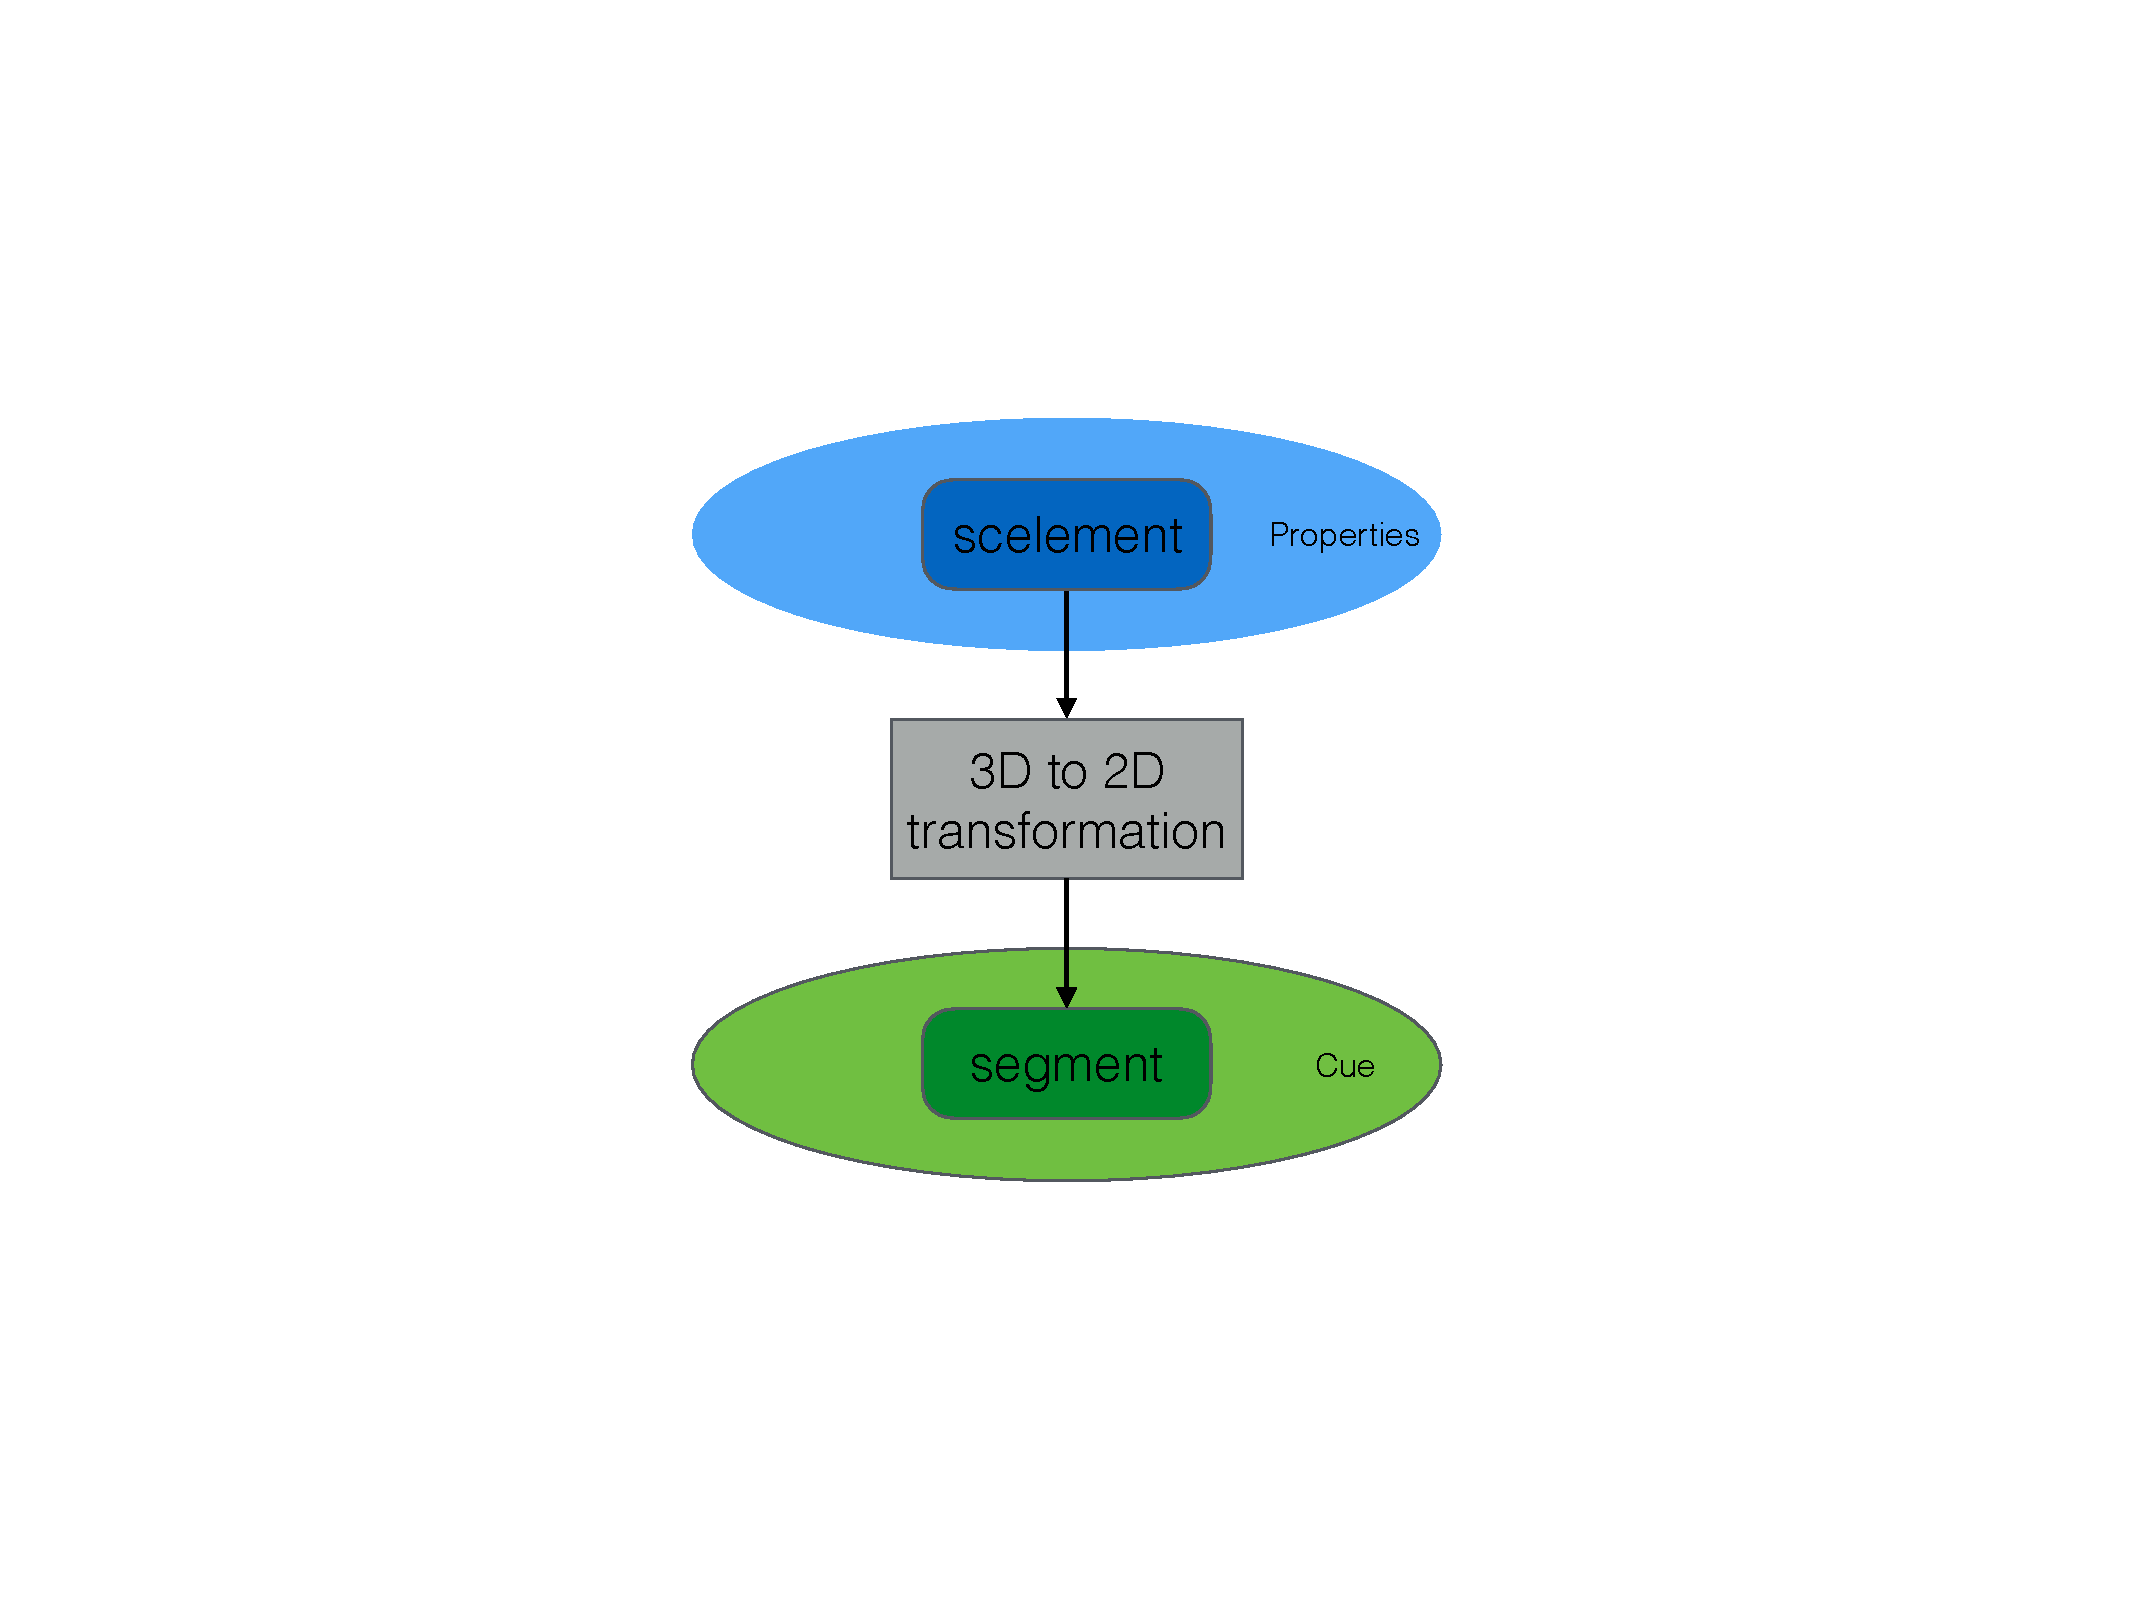
\includegraphics[width=0.5\textwidth]{model/seg_scell}
\caption{Relation between a scell and a segment}
\label{fig:scell_seg}
\end{figure}

% \textbf{Definition (Representation)} The scell can be represented as a voxel, a depth value, a 3D point/patch, or a surface normal, etc, which is denoted as $rep(sc)$.

\subsection{Consistency}
Every photograph of a 3D scene taken from a camera $C_i$ partitions the set of all possible scenes into two families, those that reproduce the photograph and those that do not. We characterize this constraint for a given shape and a given radiance assignment by the notion of \textit{consistency}.

\noindent\textbf{Definition 7 (Consistency criterion)} The consistency criterion checks whether the properties of a scell $sc$ can produce the cues observed in the corresponding segment $seg$.
\begin{align*}
consist(prop(sc), cue(seg)) = 1 &\Rightarrow \textit{consistent}\\
consist(prop(sc), cue(seg)) = 0 &\Rightarrow \textit{not consistent}
\end{align*}

\noindent\textbf{Definition 8 (Segment consistency)} Let $S$ be the scene. A scell $s\in S$ that is visible from $C_i$ is consistent with the image $I_i$ if and only if the consistency criterion is true.

\noindent\textbf{Definition 9 (Image consistency)} A scene $S$ is image consistent with image $I_i$ if any scell $\forall s\in S$ visible from the camera $C_i$ is segment consistent with this image.

\noindent\textbf{Definition 10 (Scene consistency)} A scene $S$ is scene consistent with a set of images $\{I_n\}_{n=0}^{N-1}$ if it's image consistency with each image $I_i\in \{I_n\}_{n=0}^{N-1}$ in the set.

\subsection{Formal Definition}
\noindent\textbf{Definition 11 (3D reconstruction problem)} Given a set of images $\{I_n\}_{n=0}^{N-1}$ captured by cameras $\{C_n\}_{n=0}^{N-1}$, or under a set of light sources $\{L_n\}_{n=0}^{N-1}$, find a set of scells $\{sc_m\}_{m=0}^{M-1}$ such that any scell is consistent with the visible images in the set $\{I_n\}_{n=0}^{N-1}$, \ie $\forall sc_i\in \{sc_m\}_{m=0}^{M-1}$, we the have following:
\begin{align*}
consist(prop(sc_i), cue(seg_{(i, j)})) = 1.
\end{align*}
where $seg_{(i, j)}$ is the corresponding segment of $sc_i$ in camera $C_j$. Alternatively, 3D reconstruction tries to find a set of scells $\{sc_m\}_{m=0}^{M-1}$ that are scene consistent with the image set $\{I_n\}_{n=0}^{N-1}$

\subsection{Applied Definition}
While the definition presented above gives a formal definition of the problem of 3D reconstruction, it is not necessarily applicable in a practical setting. In this section, we extend this formal definition to an approximate, yet applied version.

\noindent\textbf{Definition 12 (Consistency score)} The consistency score measures the similarity betweem a scell $sc$ and the corresponding segment $seg$.
\begin{align*}
consist(prop(sc), cue(seg)) &= x \text{, } x\in[0, 1]\\
consist(prop(sc), cue(seg)) &= 1 \Rightarrow \textit{consistent}\\
consist(prop(sc), cue(seg)) &= 0 \Rightarrow \textit{not consistent}
\end{align*}

\noindent\textbf{Definition 13 (Applied consistency criterion)} A scell $sc$ and a segment $seg$ are considered consistent if the the consistency score is above a pre-defined threshold $\epsilon$.
$$
consist(prop(sc), cue(seg)) > \epsilon
$$

% \noindent\textbf{Some more definitions} $\sum_{n\in I'}consist(prop(sc_i), cue(seg_{(i, n)}))$

\noindent\textbf{Definition 14 (Applied 3D Reconstruction Problem)} Given a set of images $\{I_n\}_{n=0}^{N-1}$ captured by cameras $\{C_n\}_{n=0}^{N-1}$, or under a set of light sources $\{L_n\}_{n=0}^{N-1}$, find a set of scells $\{sc_m\}_{m=0}^{M-1}$ such that the consistency score between the set of scells and their corresponding segments $\{seg_{(i, j)}\}_{i=0,j=0}^{M-1,N-1}$ are maximized.
$$
\mbox{maximize} \quad \sum_{j=0}^{N-1}\sum_{i=0}^{M-1} consist(prop(sc_i), cue(seg_{(i, j)}))
$$

\section{Physics-based Vision}
\label{sec:pbv}

\subsection{Radiometric terms}
\label{sec:radio_term}
Below is a list of radiometry terms, see Figure~\ref{fig:radiometry_terms} for an illustration:
\begin{itemize}
\item Solid angle ($d\omega$): 3D counterpart of angle, $d\omega=\frac{dA \cos\theta_i}{R^2}\mathit{ (steradian)}$.
\item Projected solid angle ($d\Omega$): $d\Omega = \cos\theta d\omega$.
\item Incident radiance ($\mathbf{L_i(\theta_i, \phi_i)}$): light flux received from the direction $(\theta_i, \phi_i)$ on a unit surface area, unit $\mathit{ (watt\cdot m^{-2}\cdot steradian^{-1})}$.
\item Irradiance ($\mathbf{E_i(\theta_i, \phi_i)}$): light Flux (power) incident per unit surface area from all direction, $\mathbf{E_i(\theta_i, \phi_i)}=\int_{\Omega_i} L_i(\theta_i, \phi_i) d\Omega_i \mathit{ (watt/m^2)}$.
\item Surface radiance ($\mathbf{L_r(\theta_r, \phi_r)}$): light flux emmited from a unit surface area in the direction $(\theta_r, \phi_r)$, unit $\mathit{ (watt\cdot m^{-2}\cdot steradian^{-1})}$.
\end{itemize}

\begin{figure}[!htbp]
\centering
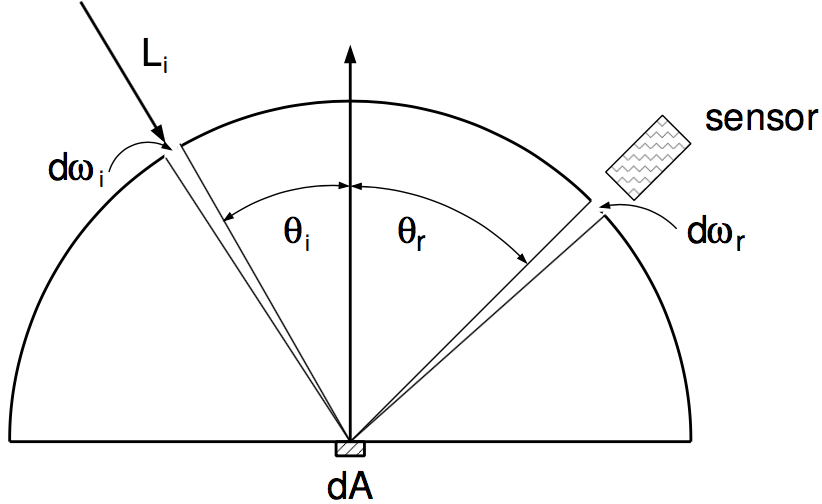
\includegraphics[width=0.5\textwidth]{model/radiometry_terms.png}
\caption{Illustration of light-matter interaction.}
\label{fig:radiometry_terms}
\end{figure}

\noindent\textbf{Definition 15 (BRDF)} the ratio of the scene radiance $\mathbf{L_r(\theta_r, \phi_r)}$ to the irradiance $\mathbf{E_i(\theta_i, \phi_i)}$, \ie $f(\theta_i, \phi_i, \theta_r, \phi_r)=\frac{L^{surface}(\theta_r, \phi_r)}{E^{surface}(\theta_i, \phi_i)}$.

\subsection{Reflectance model: microfacet model}
\label{sec:microfacet_model}
The microfacet model postulates that if a surface reflection can occur between a given light vector $\mathbf{l}$ and view vector $\mathbf{v}$, then there must exist some portion of the surface, or microfacet, with a normal aligned halfway between the $\mathbf{l}$ and $\mathbf{v}$. This ``half vector'', sometimes referred to as the microsurface normal, is thus defined as $\mathbf{h}=\frac{\mathbf{l}+\mathbf{v}}{|\mathbf{l}+\mathbf{v}|}$. A general form of the microfacet model for isotropic material is

$$
f(\mathbf{l}, \mathbf{v}) = \text{diffuse}+\frac{D(\theta_h)F(\theta_d)G(\theta_l, \theta_v)}{4\cos\theta_l\cos\theta_v}
$$

where $\theta_l$ and $\theta_v$ are the angles of incidence of $\mathbf{l}$ and $\mathbf{v}$ vectors with respect to the normal $\theta_h$ is the angle between the normal and the half vector, and $\theta_d$ is the ``difference'' angle between $\mathbf{l}$ and the half vector.

The diffuse term is a function of unknown form. Lambert diffuse is often assumed and is represented by a constant value. For the specular term, $D$ is the microfacet distribution function and is responsible for the shape of the specular peak, $F$ is the Fresnel reflection coefficient, and $G$ is the geometric attenuation or shadowing factor.

\subsection{Image formation: radiometric perspective}
This section discusses the radiometric perspective of image formation. Specifically, we discuss the contributing factors that determine the pixel intensity of an image.

\subsubsection{Light-matter interaction}
The relation between the incoming illumination and reflected light is modelled using the \textit{bidirectional reflectance distribution function} (BRDF), refer to the Appendix~\ref{sec:radio_term} for definitions of radiometric terms.
\begin{figure}[!htbp]
\centering
\begin{tikzpicture}[node distance=2cm, auto]
\node (light_rad) [data] {Incident Radiance};
\node (material) [model, right of=light_rad, xshift=2cm] {Material};
\node (scene_rad) [data, right of=material, xshift=2cm] {Scene Radiance};
\draw [arrow] (light_rad) -- (material);
\draw [arrow] (material) -- (scene_rad);
\end{tikzpicture}
\caption{The light-matter interaction. Scene radiance is linear related to incident radiance.}
\label{fig:light_matter_interact}
\end{figure}

As we can see from the definition of BRDF, scene radiance is a function of BRDF given a fixed incident radiance. BRDF is a bidirectional function, which depends on both incoming and outgoing directions. It can be simplified under specific reflectance models. For instance, BRDF can be simplified as \textit{Diffuse albedo} or surface albedo when using Lambertian reflectance, which is the proportion of incident light that is reflected by the surface.
% It should be noted that albedo is not an intrinsic property of a surface. Instead, for any surface, the albedo depends on the spectral and angular distributions of the incident light.

\subsubsection{Light sensor interaction}
A common assumption made in vision community is that radiance is constant as it propagates along a ray. Therefore, the scene radiance is the same as the radiance passing through the lens, which is the same as the radiance received by the sensor. Since image irradiance is the radiance accumulated on a unit surface area, it follows that image irradiance is linear related to the scene radiance. Thus, the relation between \textit{scene radiance} and \textit{image irradiance} is linear.
\begin{figure}[!ht]
\centering
\begin{tikzpicture}[node distance=2cm, auto]
\node (scene_rad) [data] {Scene Radiance};
\node (lens) [model, right of=scene_rad, xshift=2cm] {Lens};
\node (irradiance) [data, right of=lens, xshift=2cm] {Image Irradiance};
\draw [arrow] (scene_rad) -- (lens);
\draw [arrow] (lens) -- (irradiance);
\end{tikzpicture}
\caption{The light-sensor interaction. Image irradiance is linearly related to scene radiance.}
\label{fig:light_lens_interact}
\end{figure}

\subsubsection{Irradiance-intensity conversion}
The camera response function relating image irradiance at the image plane to measured pixel intensity values is a non-linear mapping. It is common to assume that intensity is linear related to image irradiance in many vision algorithms. A linear relation can be retrieved by radiometric calibration.
\begin{figure}[!htbp]
\centering
\begin{tikzpicture}[node distance=2cm, auto]
\node (irradiance) [data] {Image Irradiance};
\node (response) [model, right of=irradiance, xshift=2cm] {NL-response};
\node (intensity) [data, right of=response, xshift=2cm] {Intensity};
\draw [arrow] (irradiance) -- (response);
\draw [arrow] (response) -- (intensity);
\end{tikzpicture}
\caption{The camera response function is typically non-linear. Thus pixel intensity if non-linear with respect to irradiance. However, this can be corrected by radiometric calibration. More often, it is assumed that pixel intensity is linearly related to image irradiance in many vision algorithms.}
\label{fig:light_sensor_interact}
\end{figure}

\section{Material of real-world objects}
\label{sec:real_world_dataset}
\begin{table}[!hbtp]
  \centering
  \begin{tabular}{*{9}{c}}
  \multicolumn{3}{l}{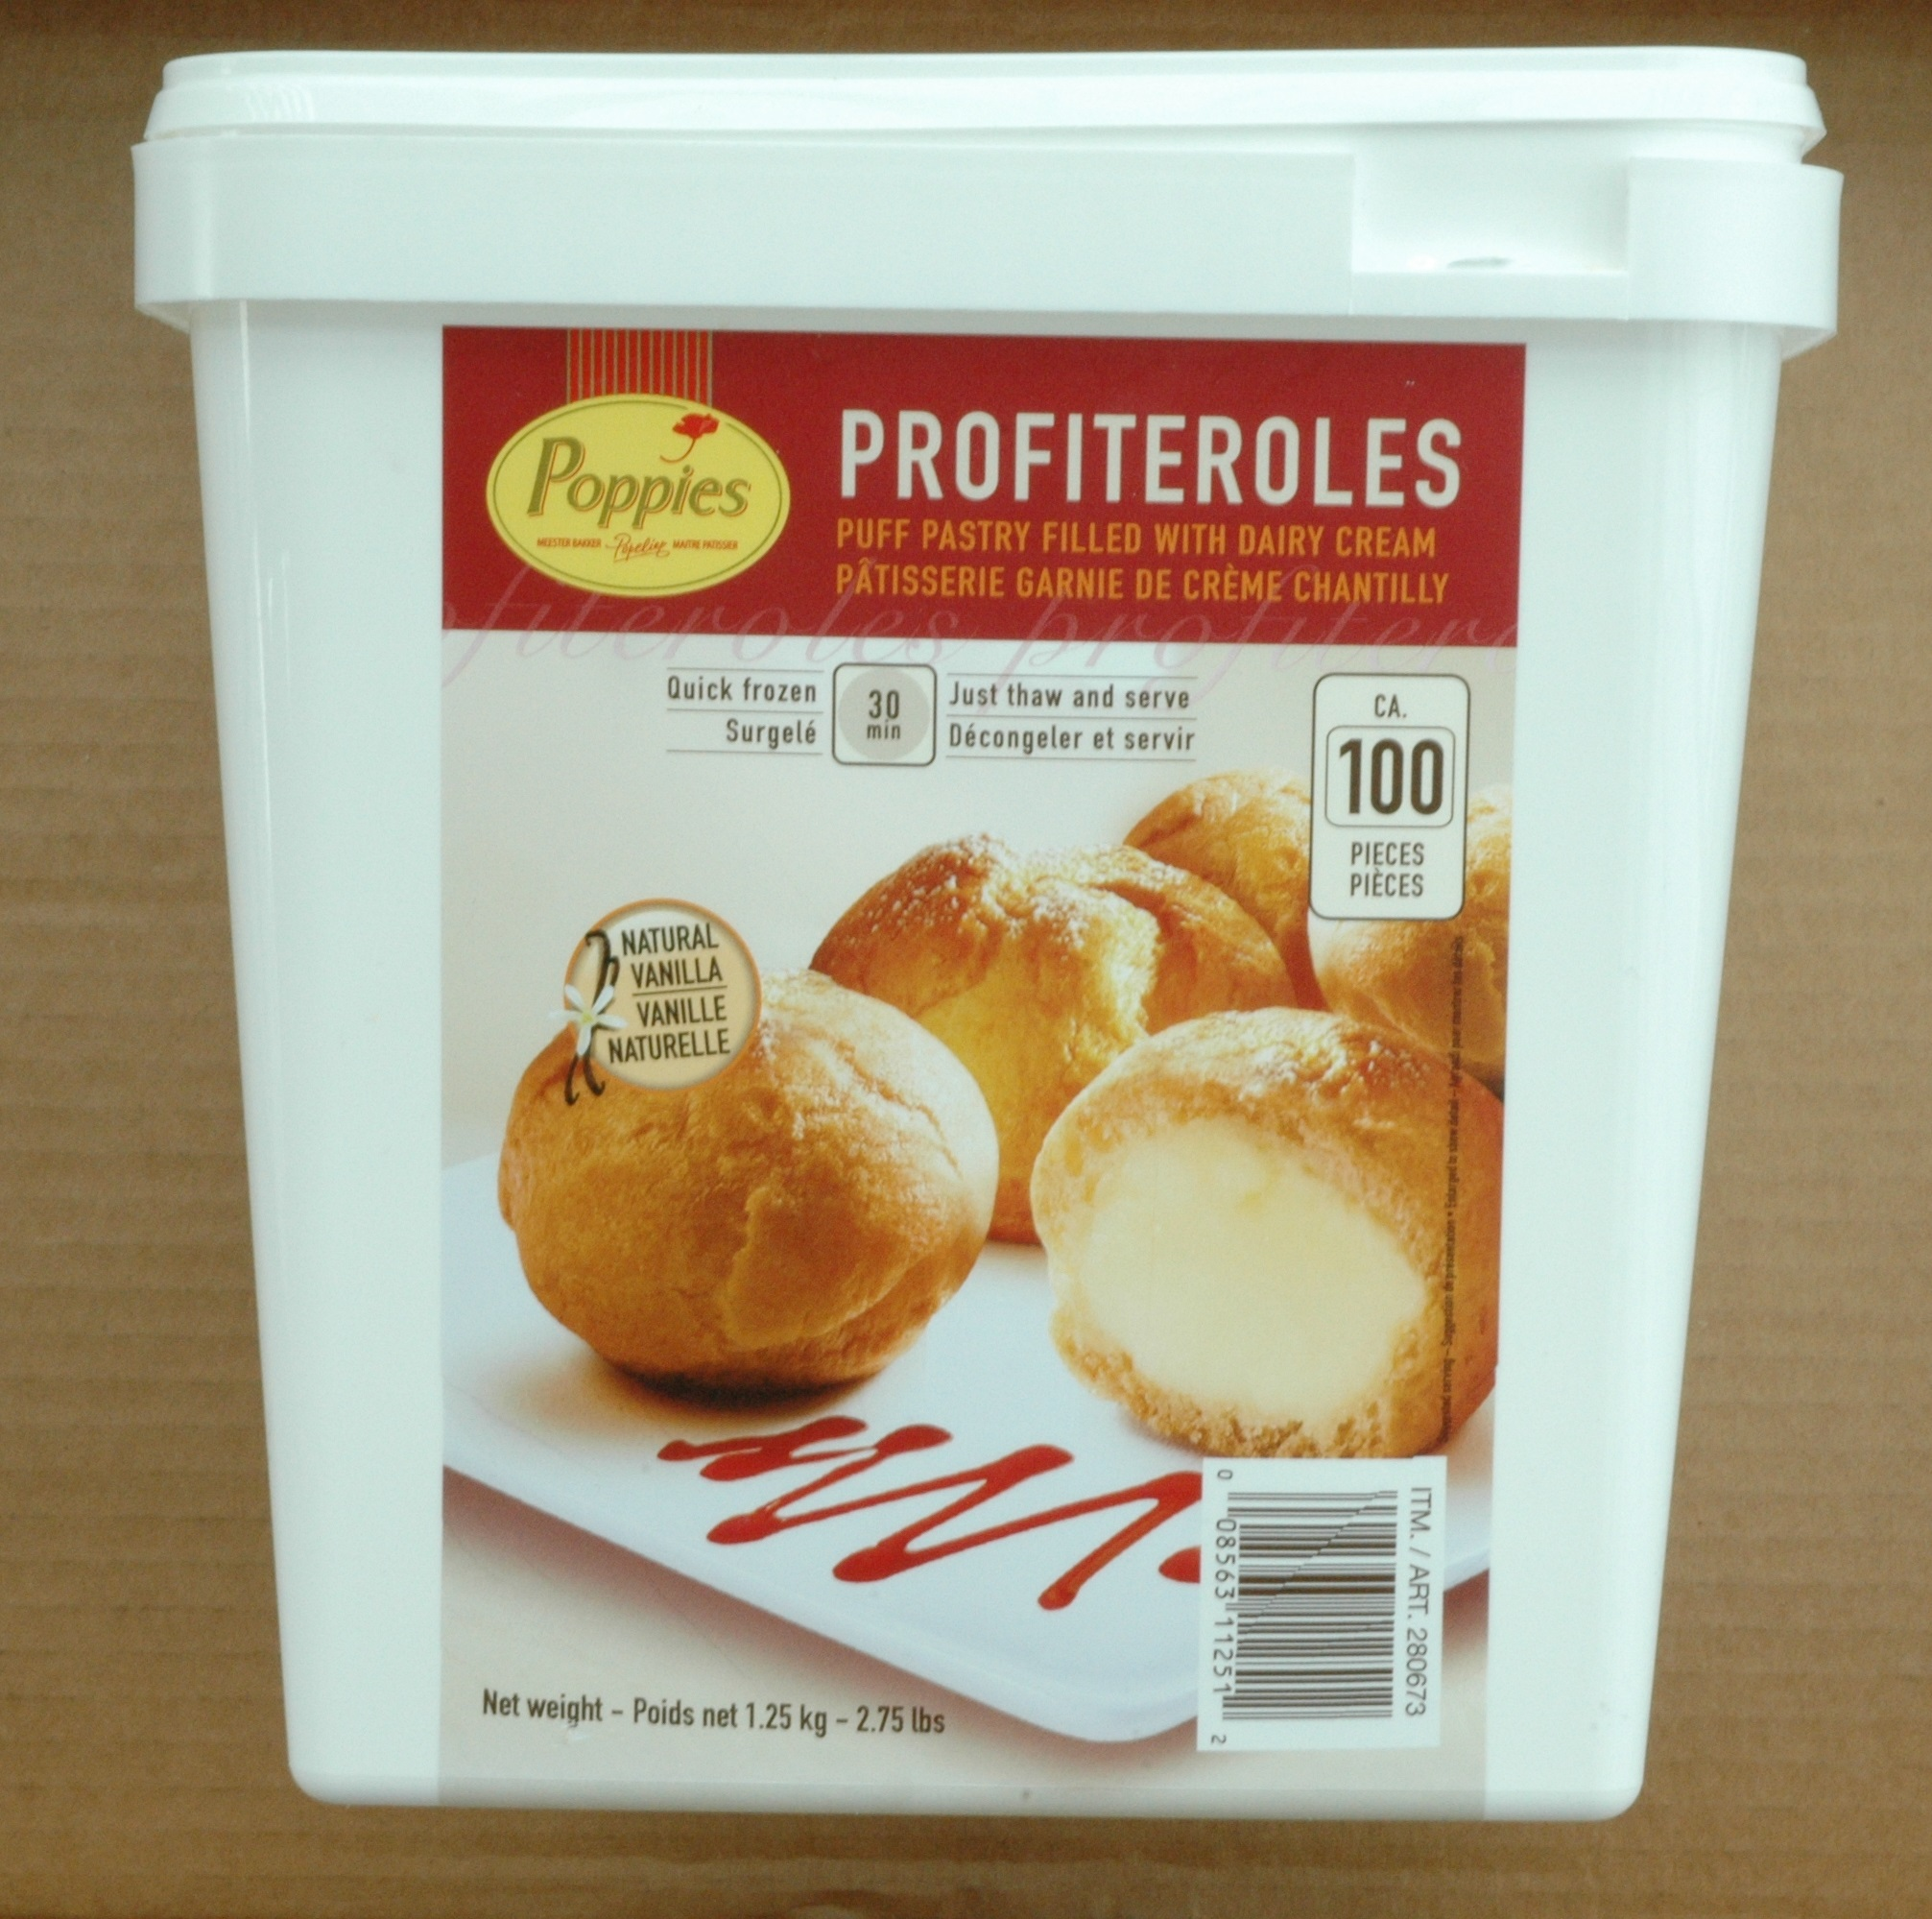
\includegraphics[width=0.33\textwidth]{interp/real_world_img/box/box}} &
  \multicolumn{3}{l}{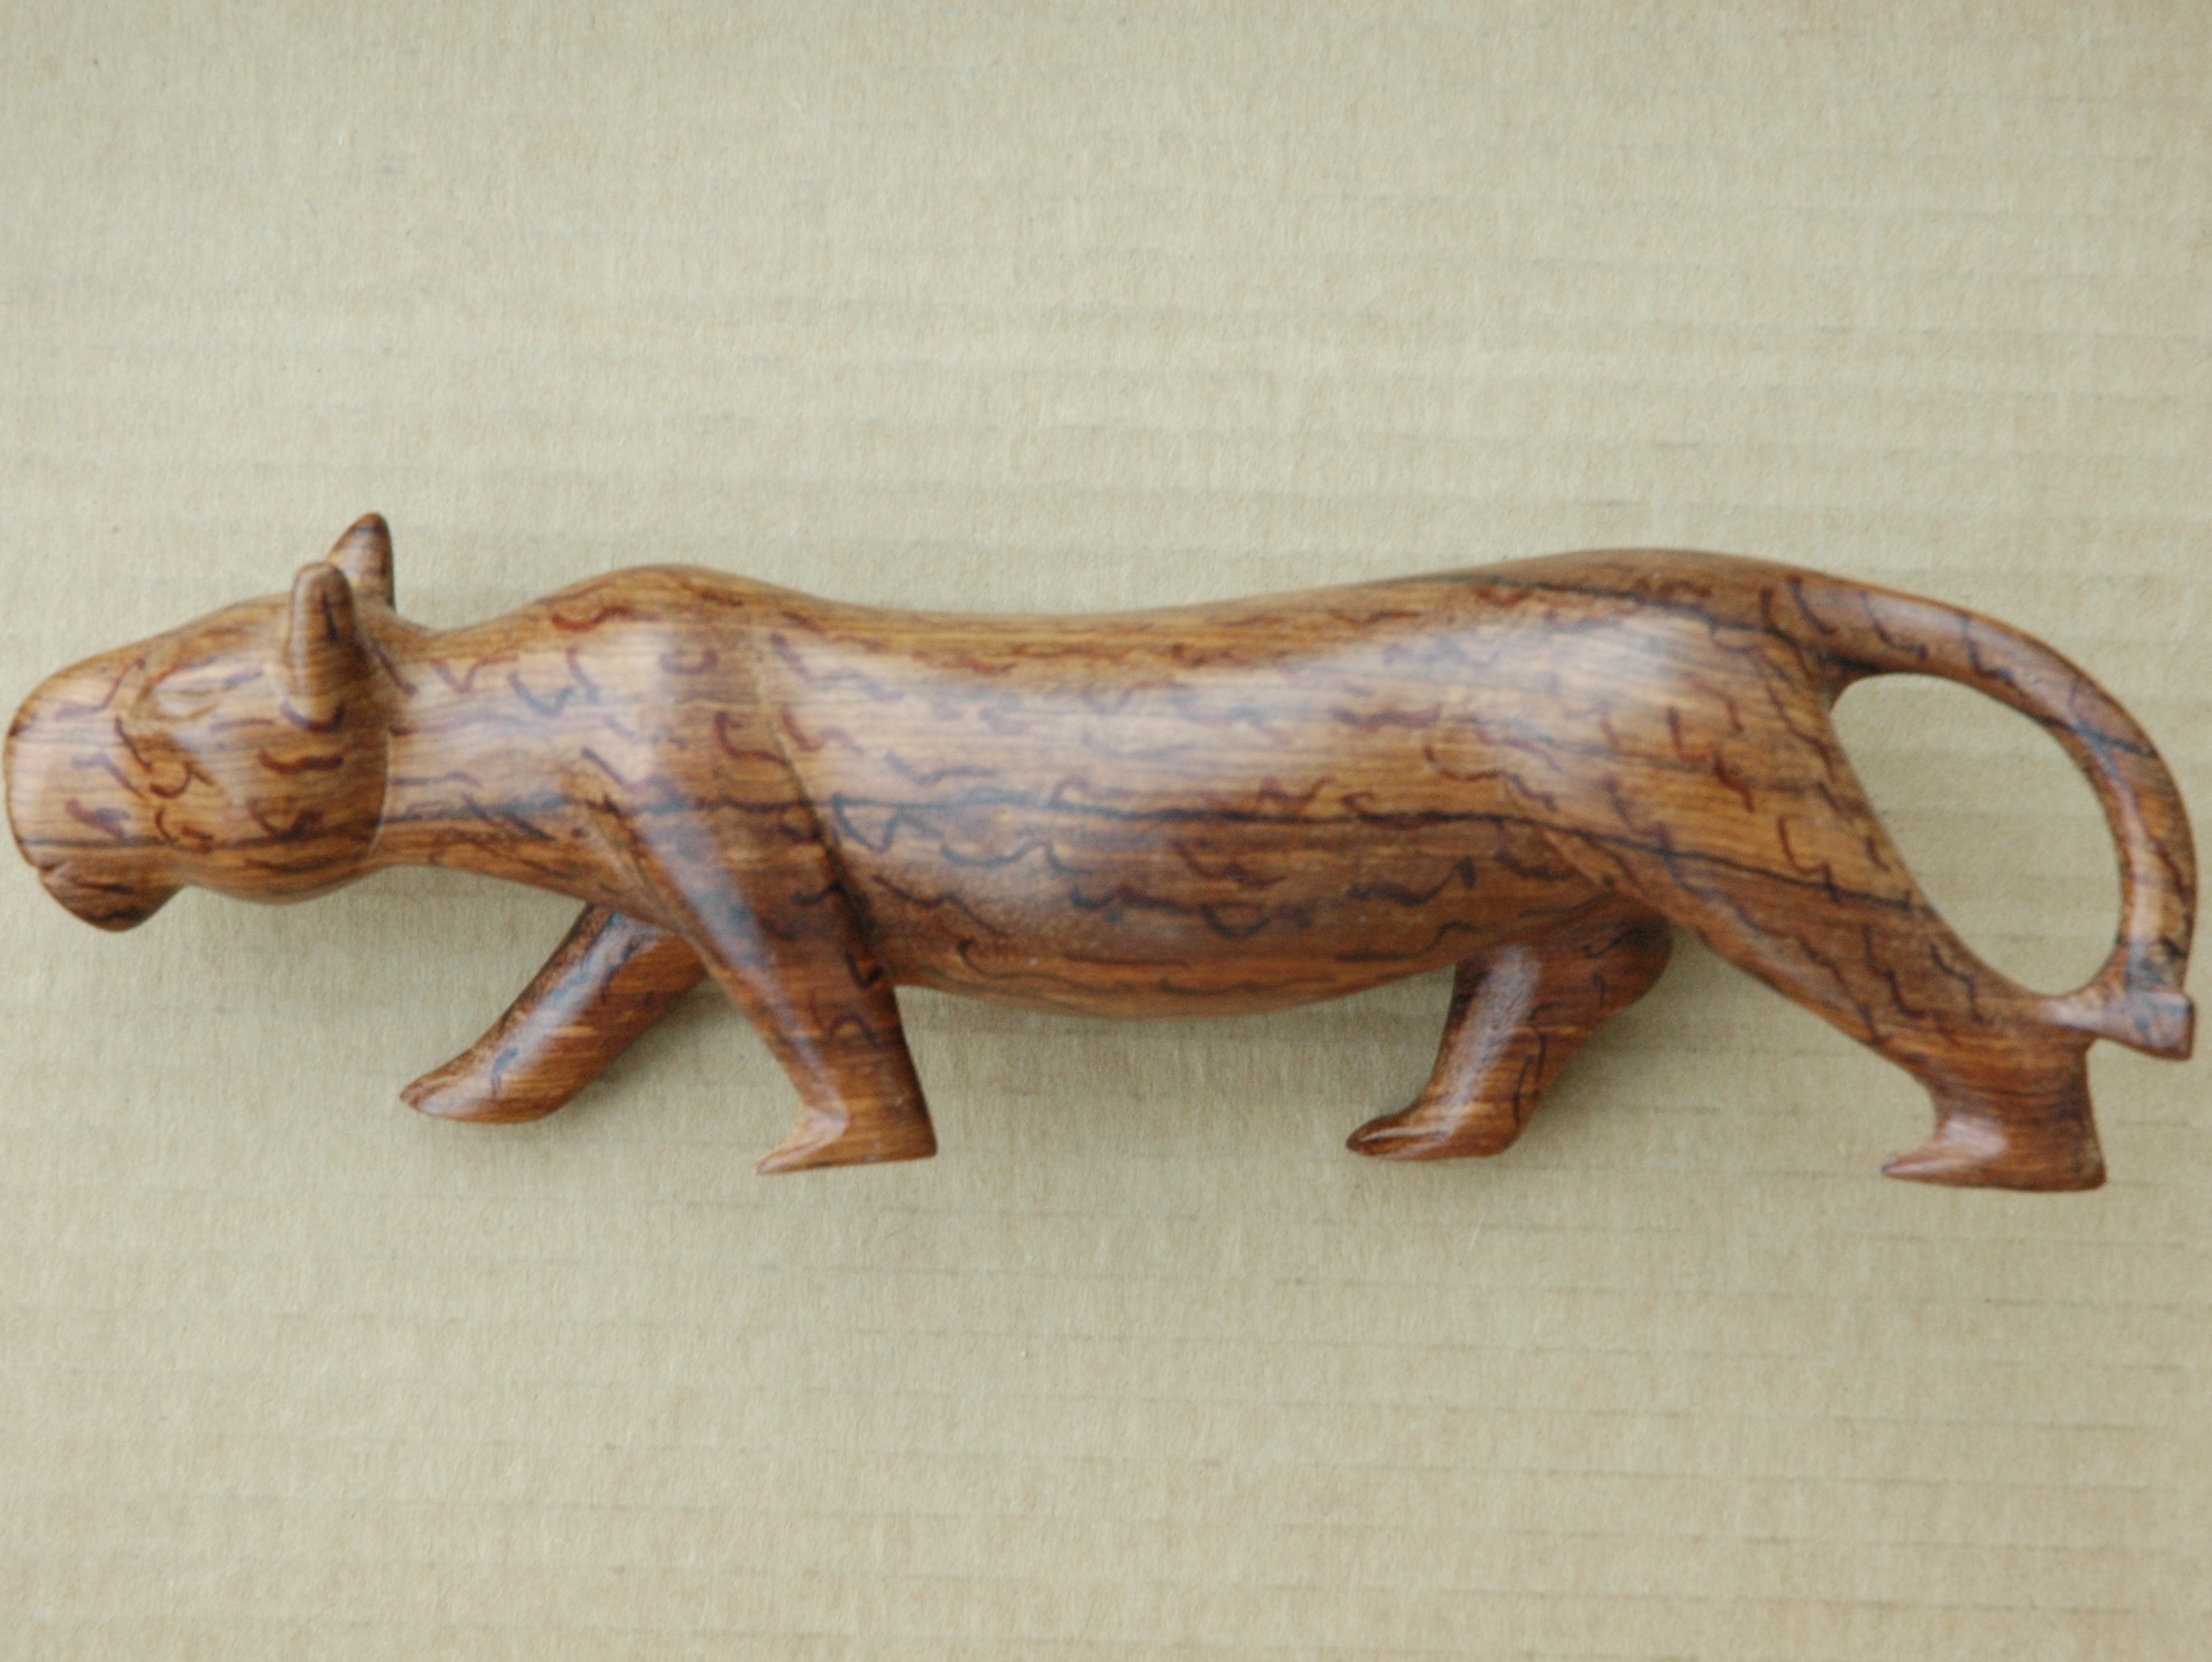
\includegraphics[width=0.33\textwidth]{interp/real_world_img/cat0/cat0}} &
  \multicolumn{3}{l}{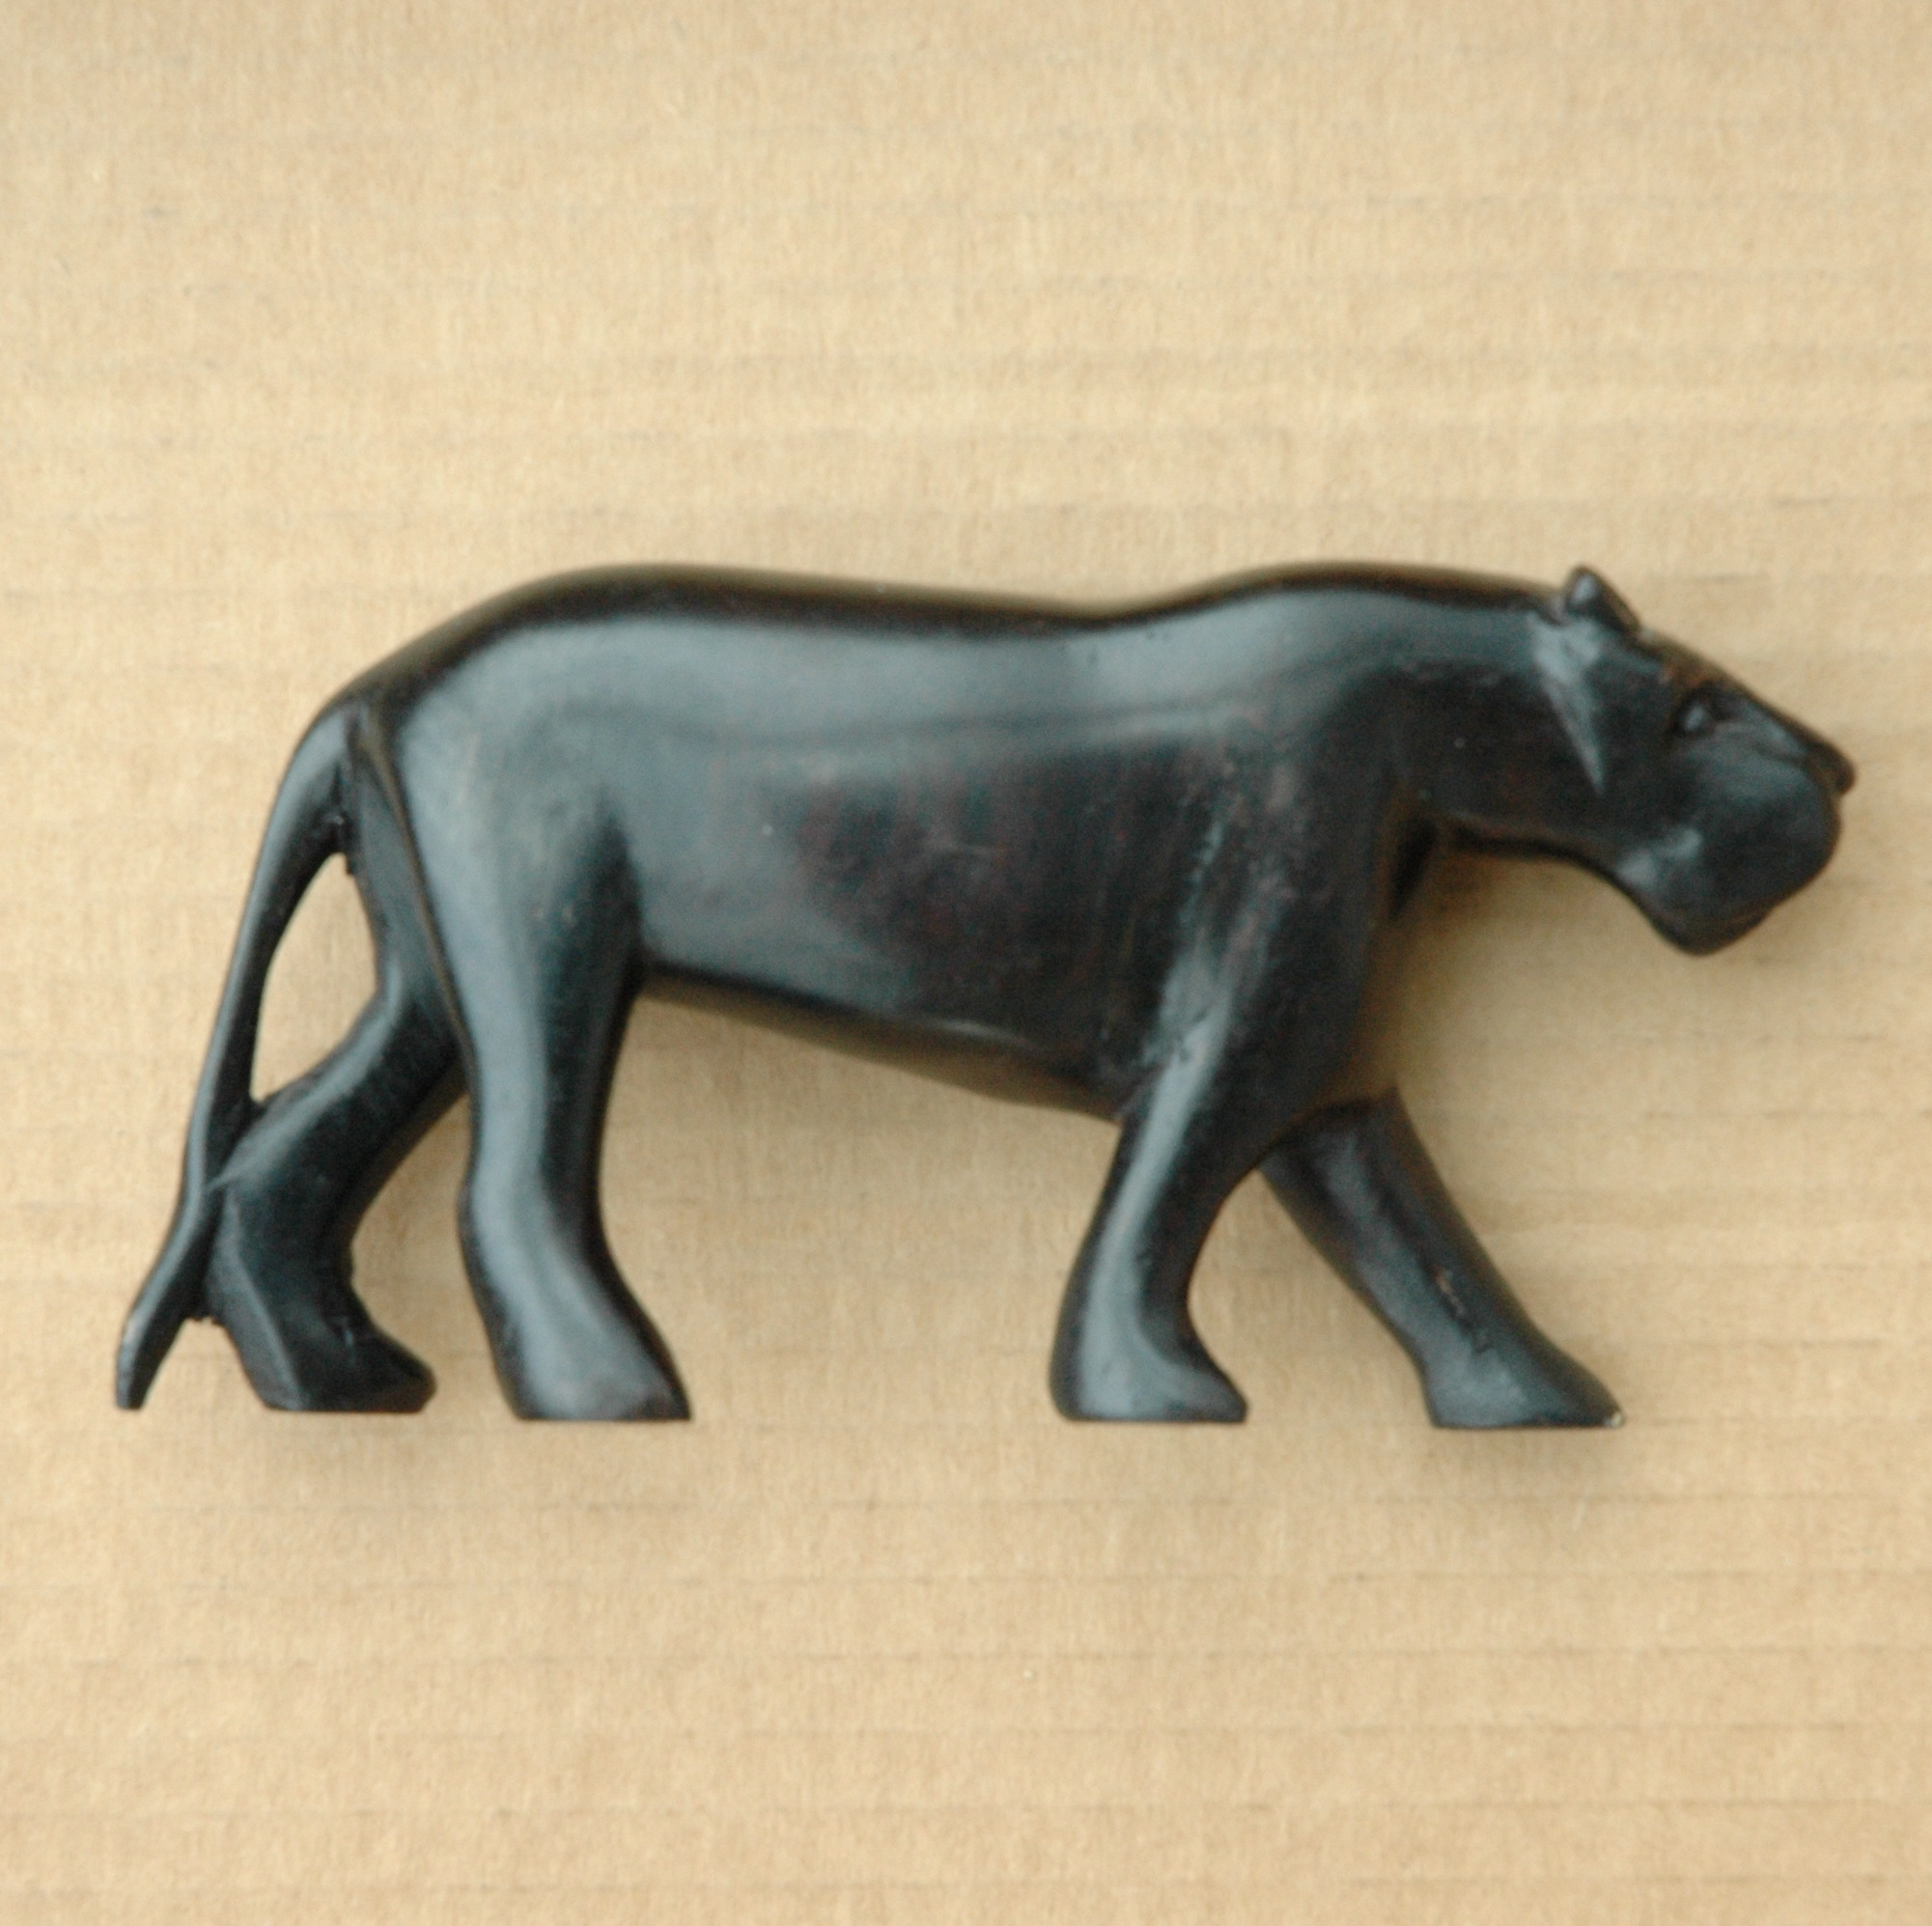
\includegraphics[width=0.33\textwidth]{interp/real_world_img/cat1/cat1}}\\
  % \includegraphics[width=0.1\textwidth]{interp/real_world_img/box/base_00} &
  % \includegraphics[width=0.1\textwidth]{interp/real_world_img/box/base_01} & 
  % \includegraphics[width=0.1\textwidth]{interp/real_world_img/box/base_02} &
  % \includegraphics[width=0.1\textwidth]{interp/real_world_img/cat0/base_00} & 
  % \includegraphics[width=0.1\textwidth]{interp/real_world_img/cat0/base_01}& &
  % \includegraphics[width=0.1\textwidth]{interp/real_world_img/cat1/base_00} &\\
  \multicolumn{3}{c}{(a). box} & \multicolumn{3}{c}{(b). cat0} & \multicolumn{3}{c}{(c). cat1} \\
  \multicolumn{3}{l}{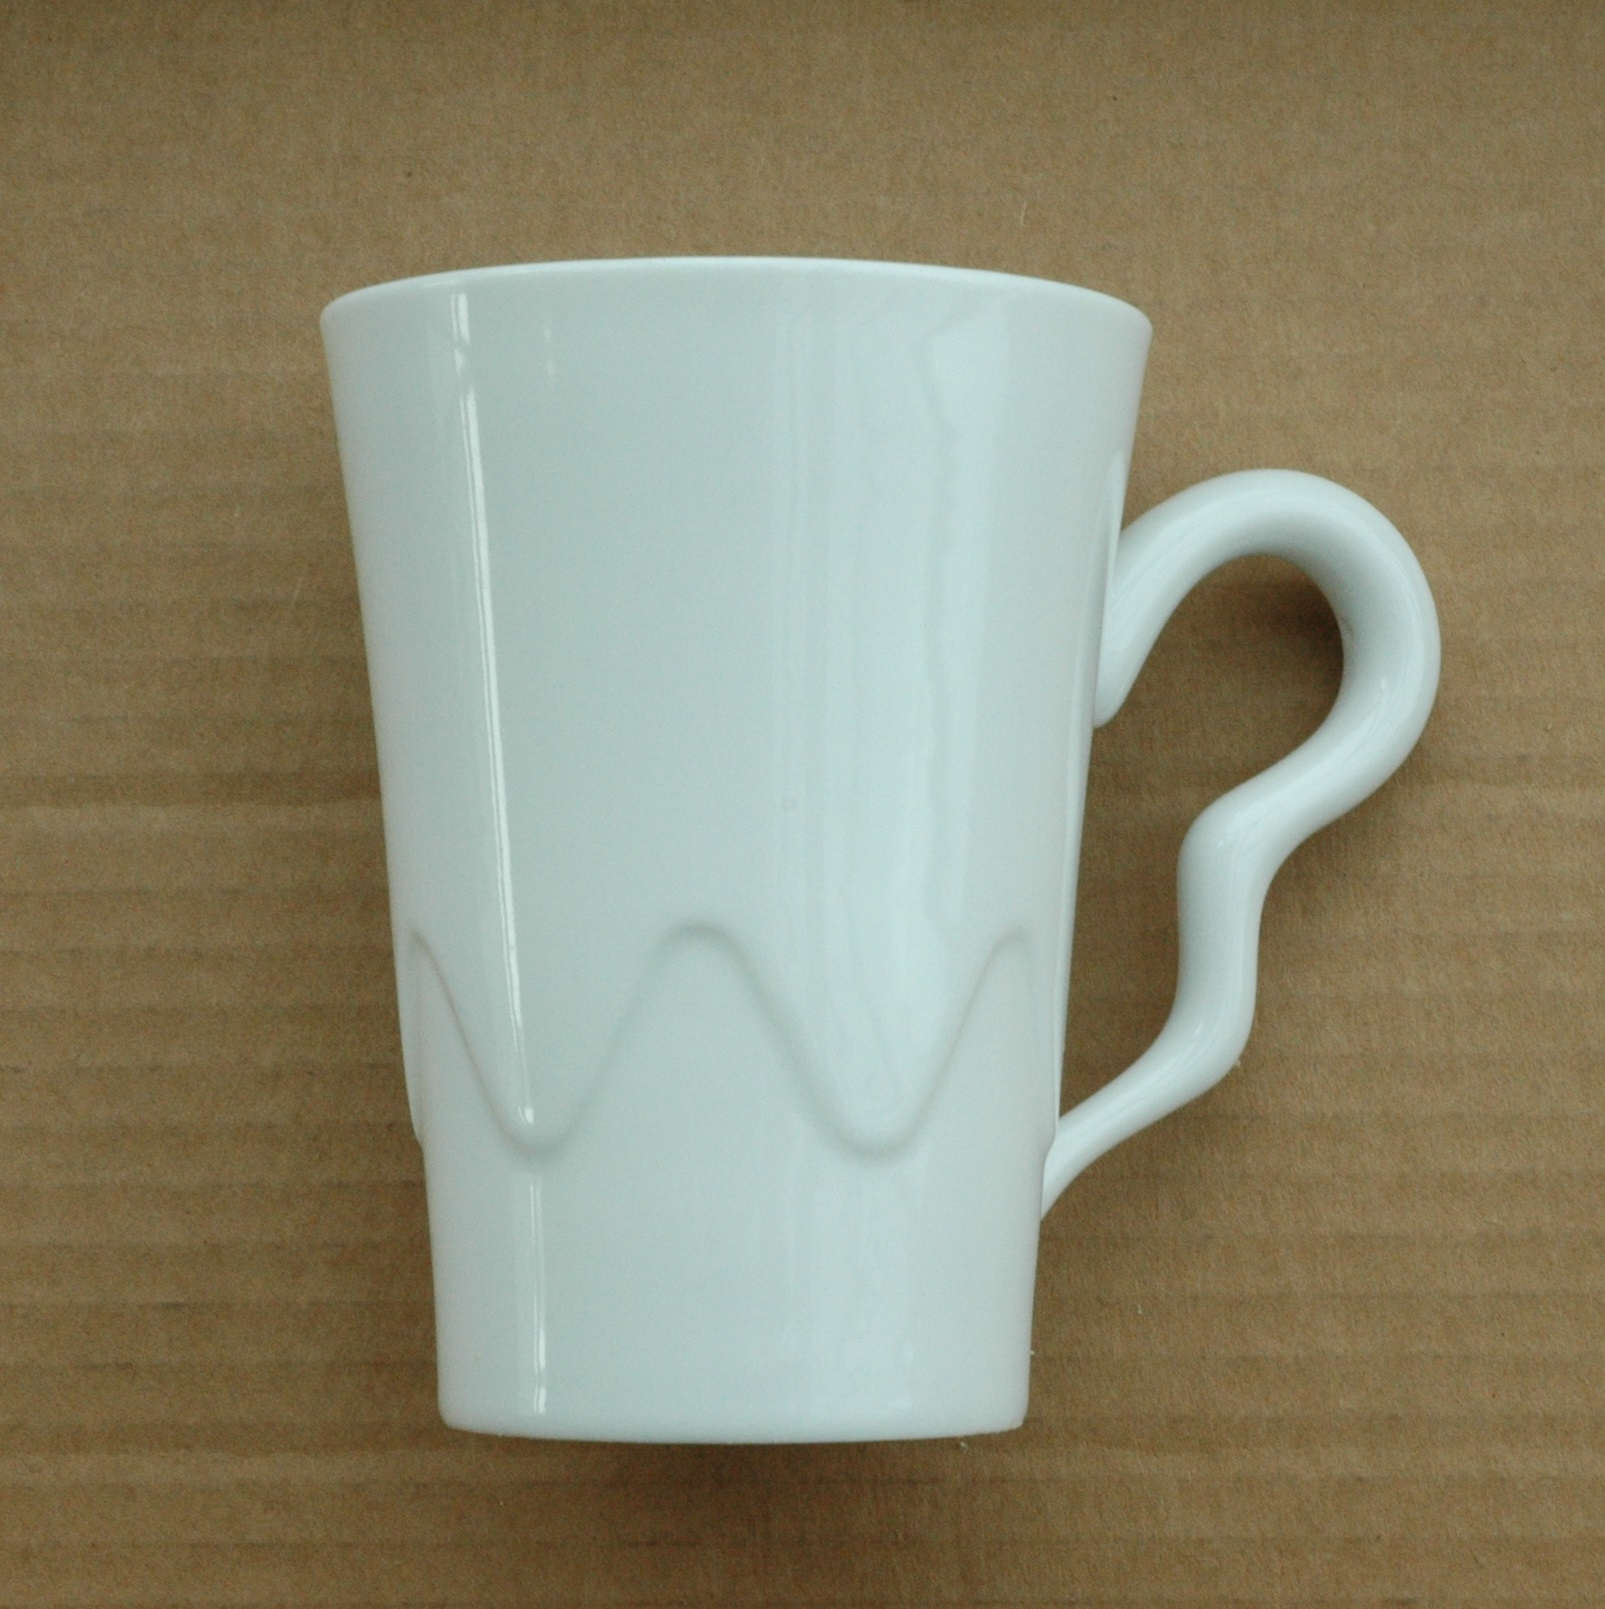
\includegraphics[width=0.33\textwidth]{interp/real_world_img/cup/cup}} &
  \multicolumn{3}{l}{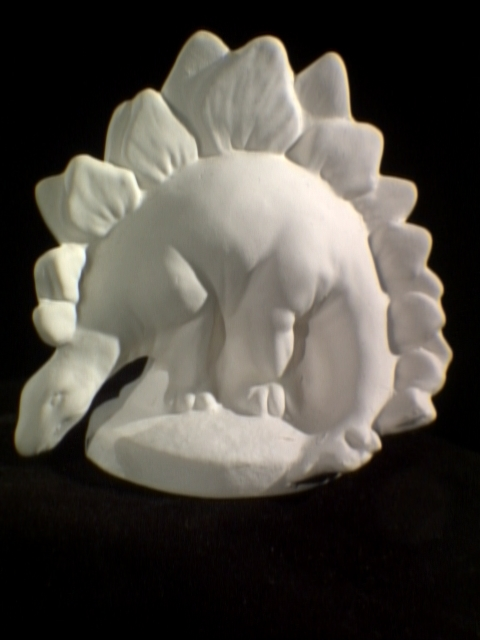
\includegraphics[width=0.33\textwidth]{interp/real_world_img/dino/dino}} &
  \multicolumn{3}{l}{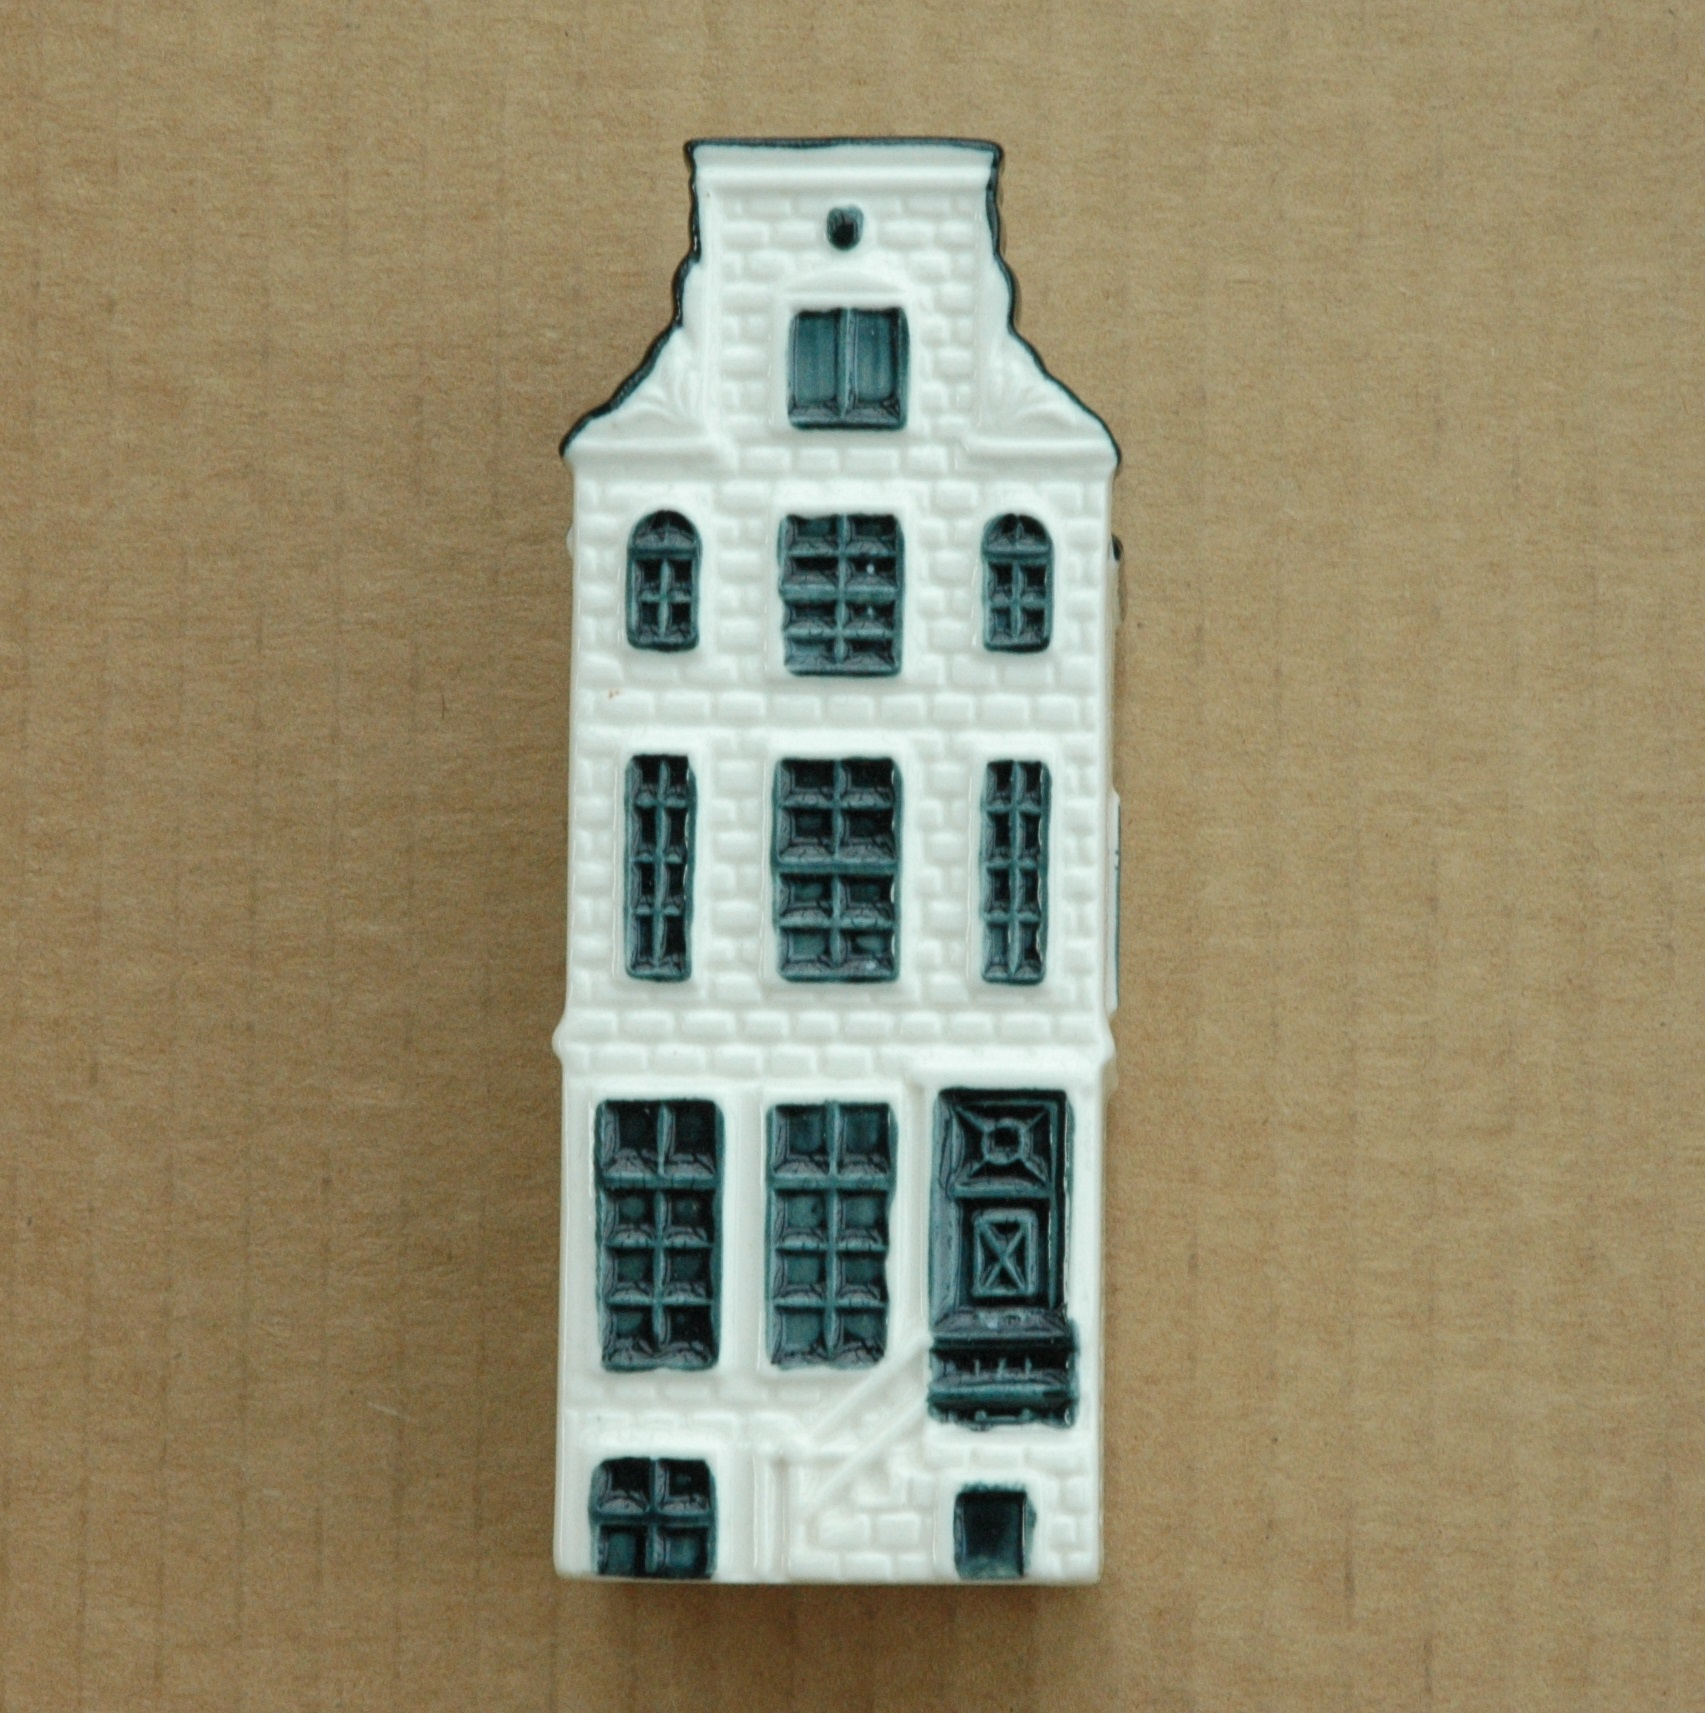
\includegraphics[width=0.33\textwidth]{interp/real_world_img/house/house}}\\
  % \includegraphics[width=0.1\textwidth]{interp/real_world_img/cup/base_00} & & &
  % \includegraphics[width=0.1\textwidth]{interp/real_world_img/dino/base_00} & 
  % \includegraphics[width=0.1\textwidth]{interp/real_world_img/dino/base_01} & 
  % \includegraphics[width=0.1\textwidth]{interp/real_world_img/dino/base_02} &
  % \includegraphics[width=0.1\textwidth]{interp/real_world_img/house/base_00} &
  % \includegraphics[width=0.1\textwidth]{interp/real_world_img/house/base_01} & \\
  \multicolumn{3}{c}{(d). cup} & \multicolumn{3}{c}{(e). dino} & \multicolumn{3}{c}{(f). house} \\
  \multicolumn{3}{l}{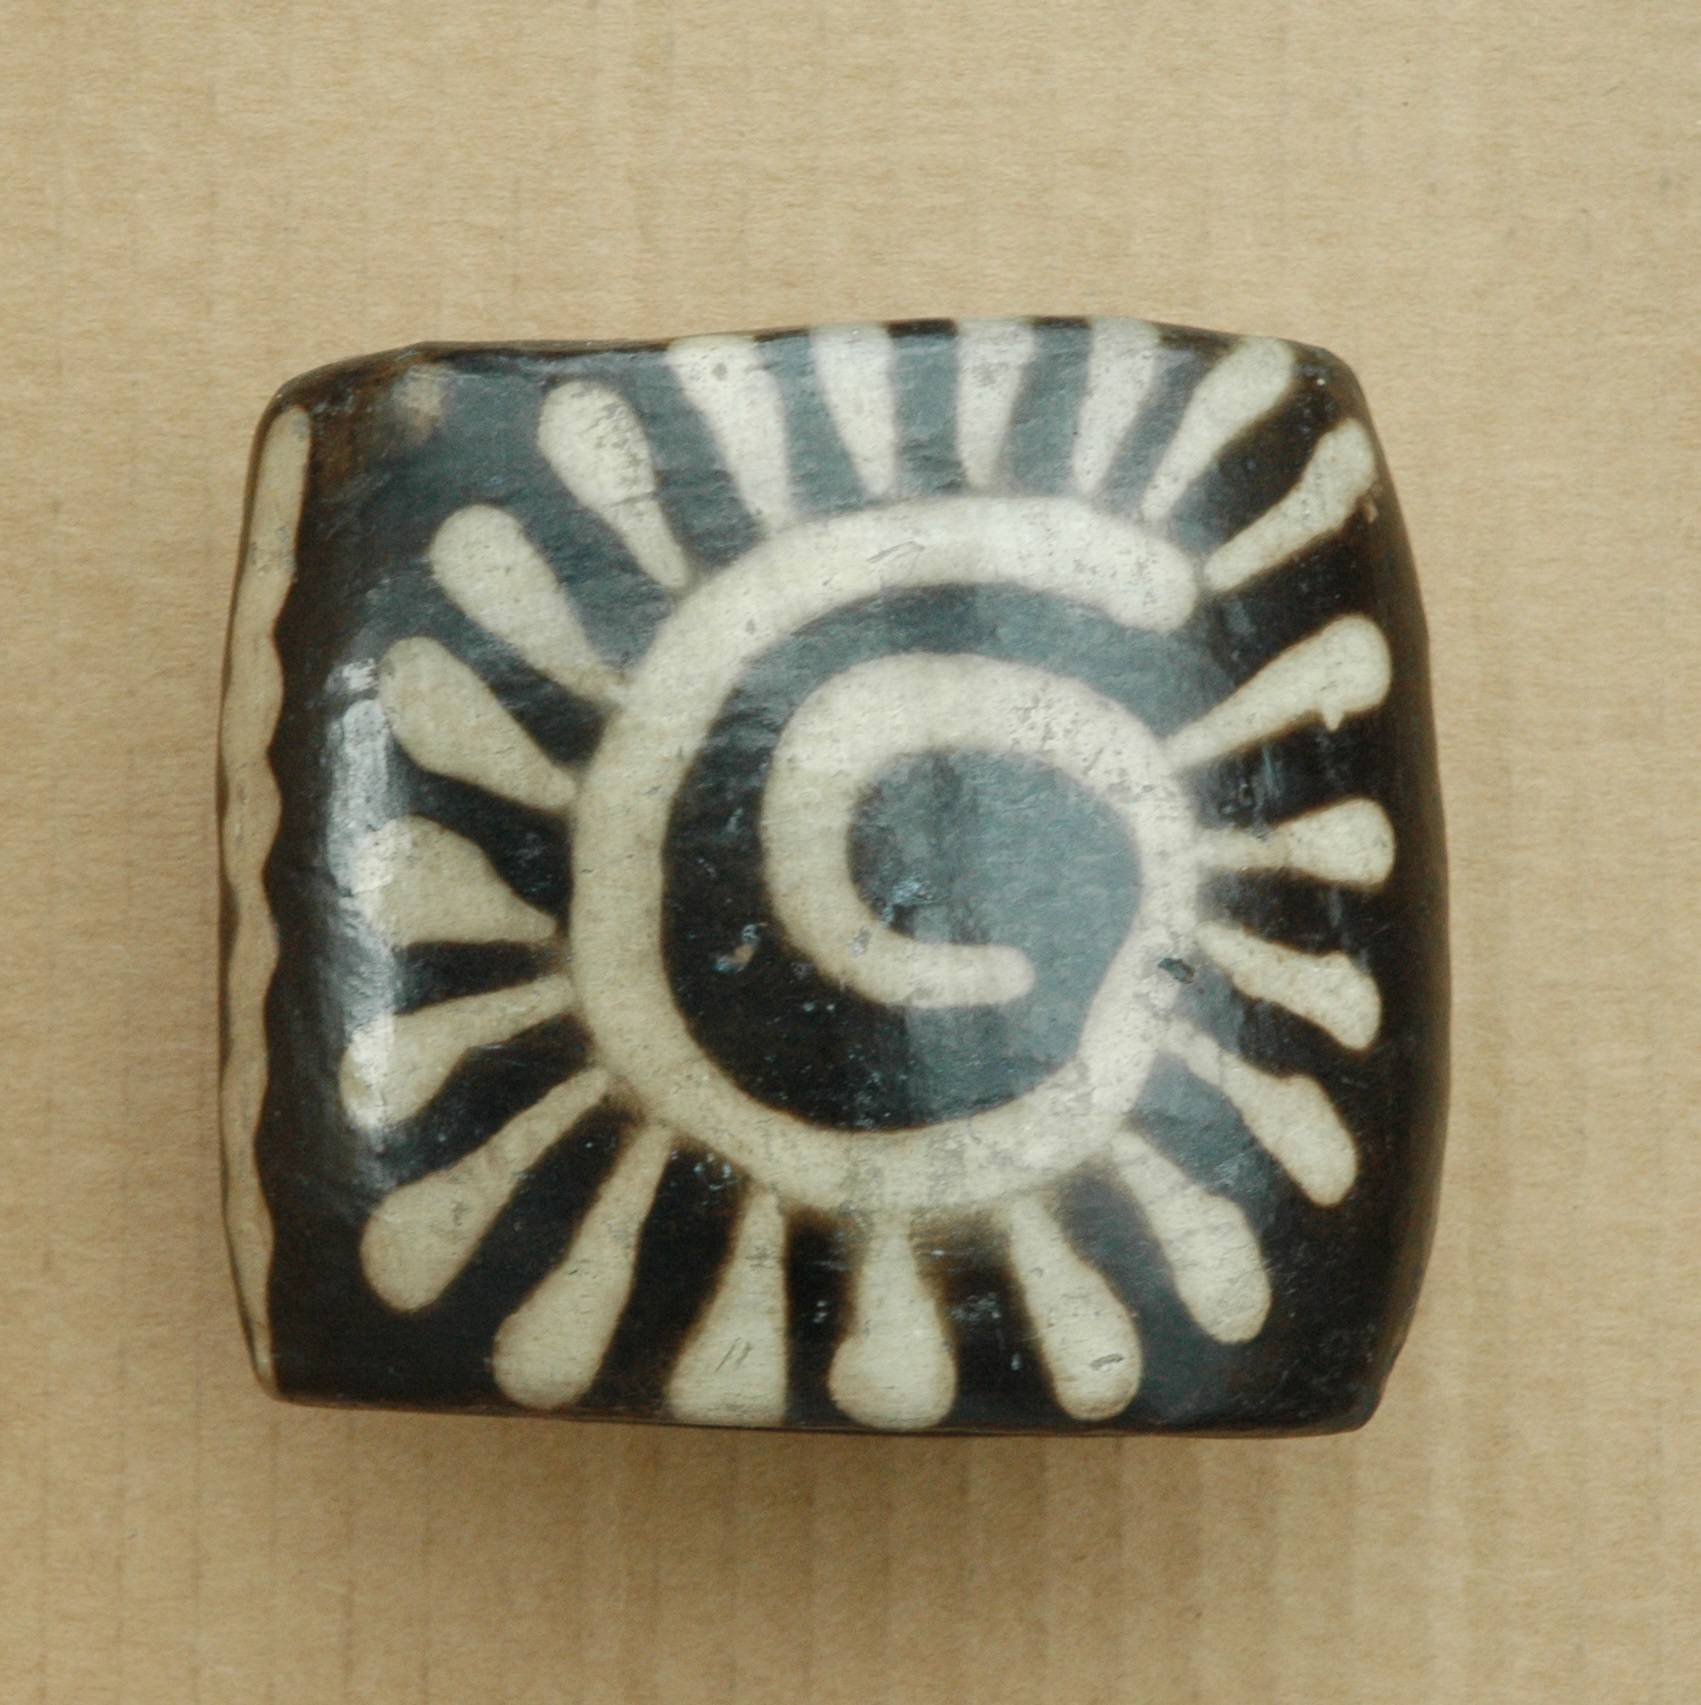
\includegraphics[width=0.33\textwidth]{interp/real_world_img/pot/pot}} &
  \multicolumn{3}{l}{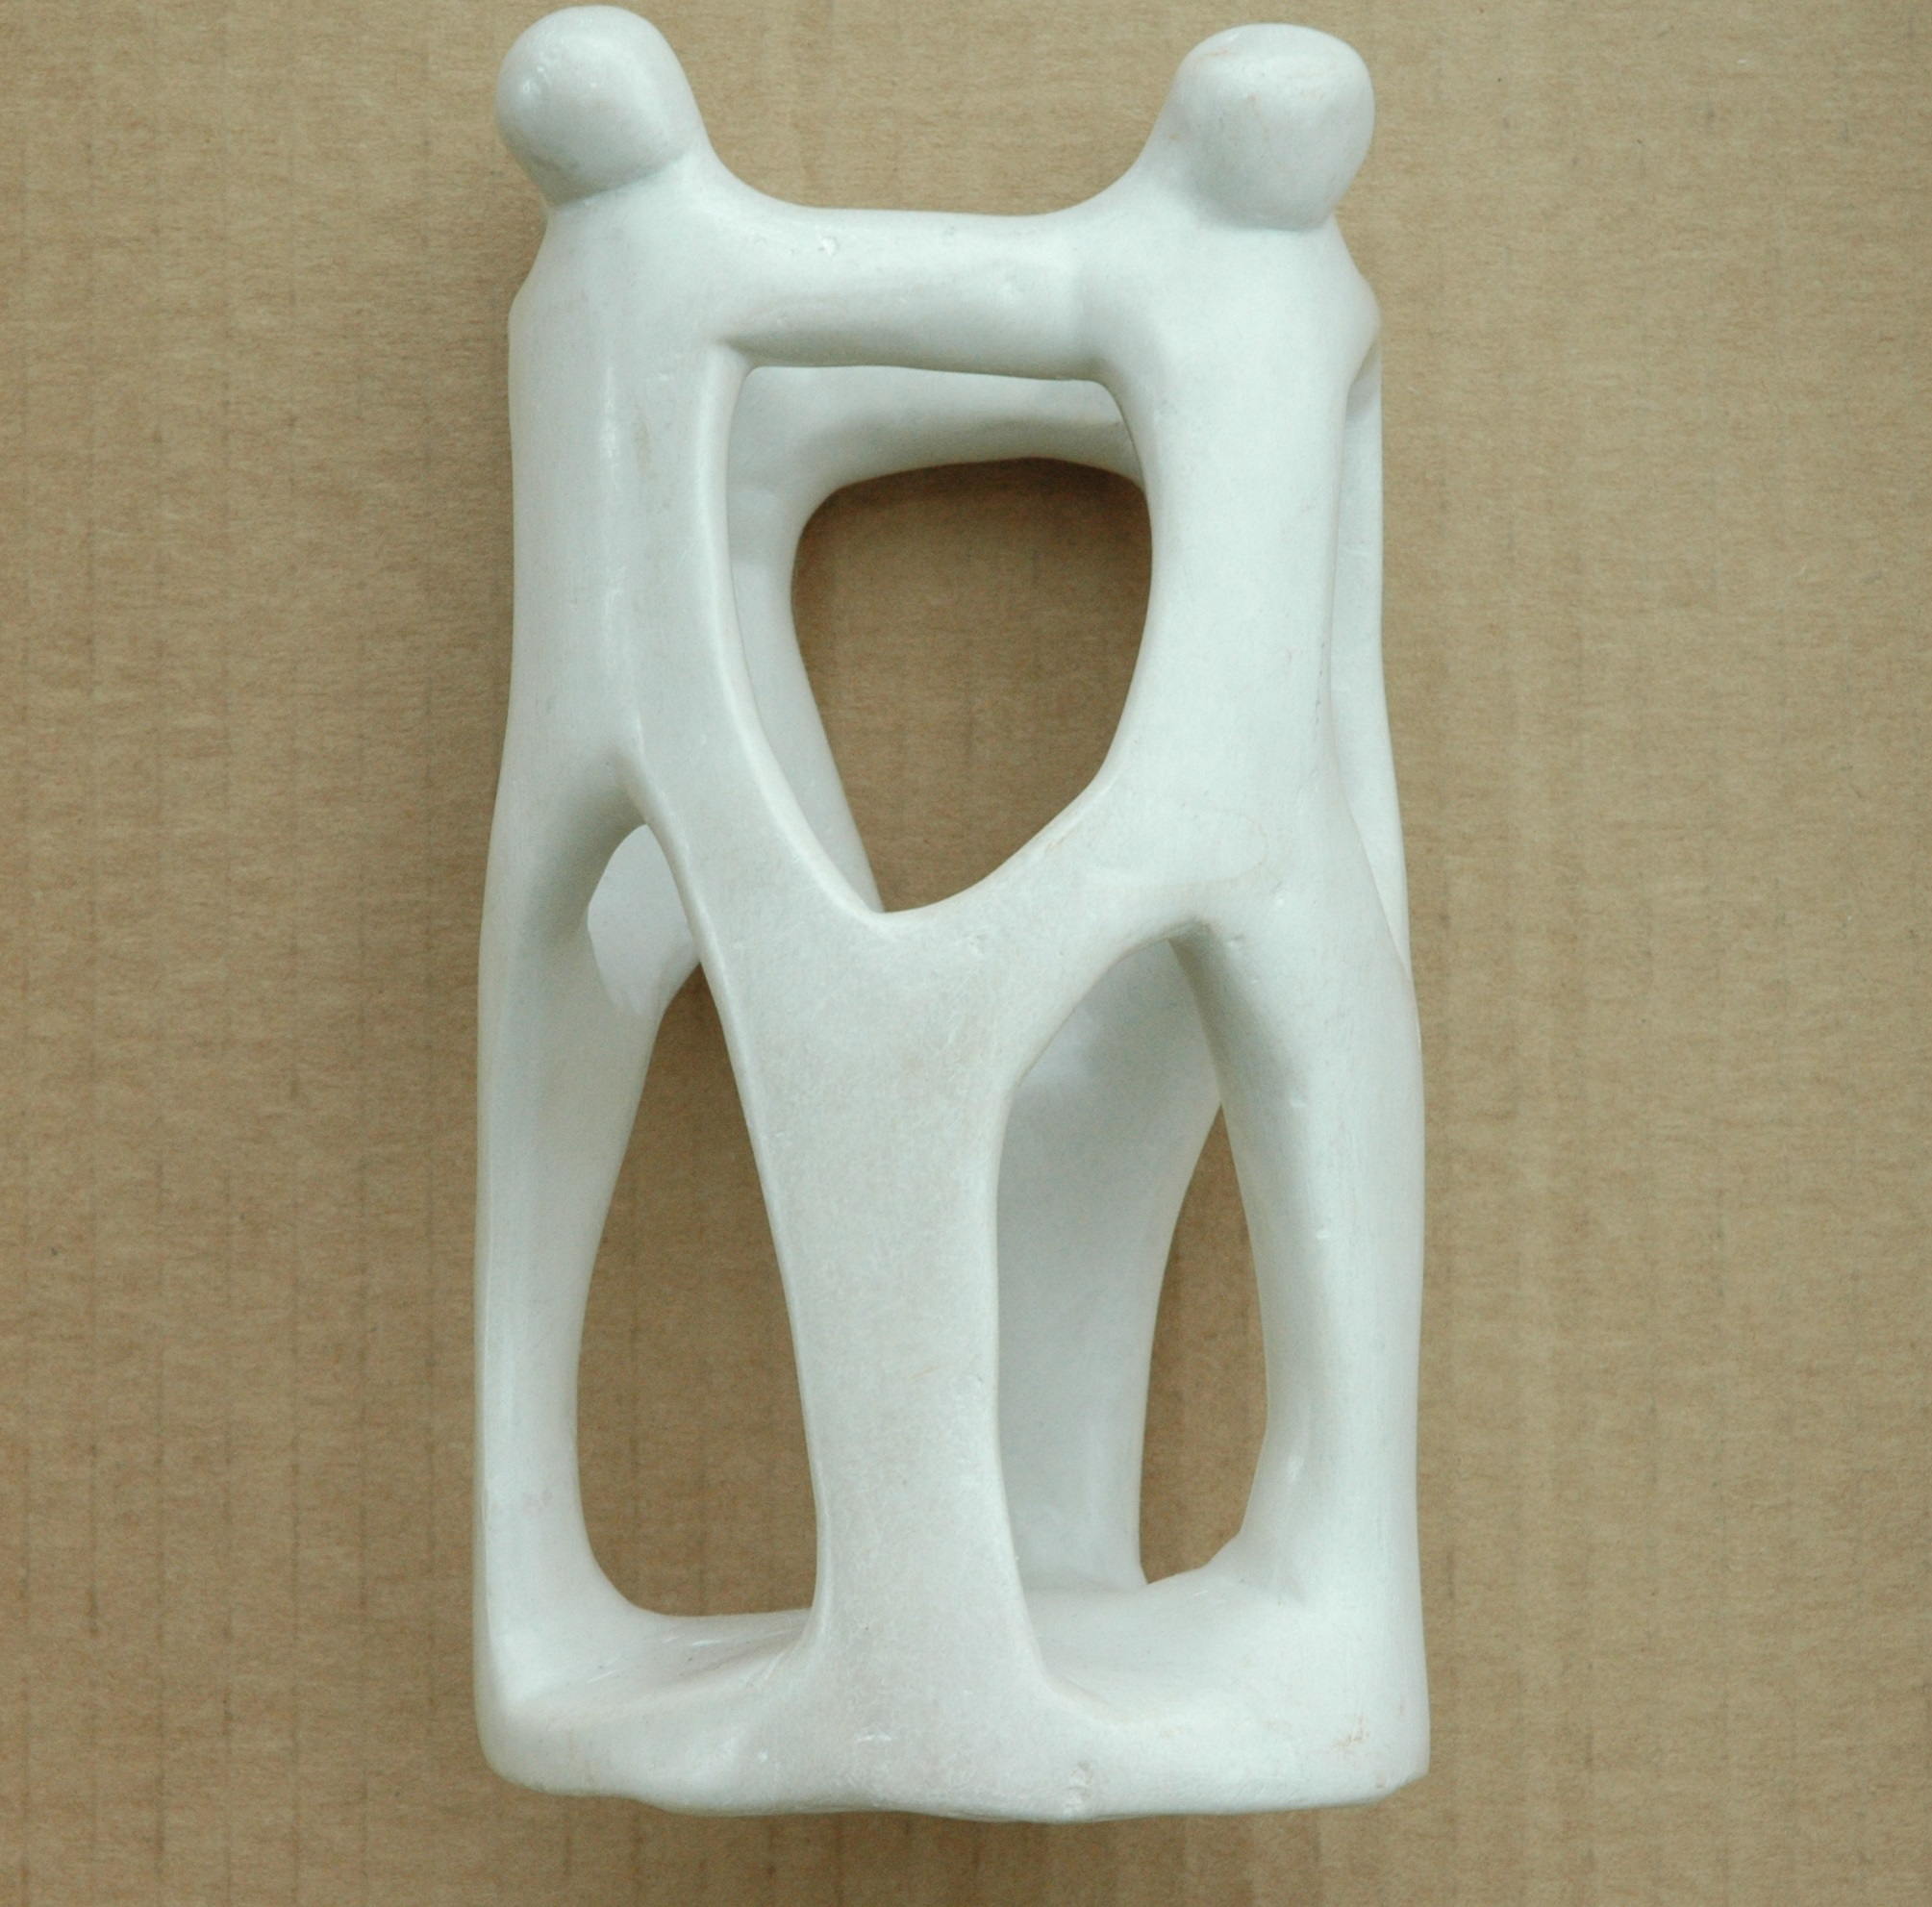
\includegraphics[width=0.33\textwidth]{interp/real_world_img/statue/statue}} &
  \multicolumn{3}{l}{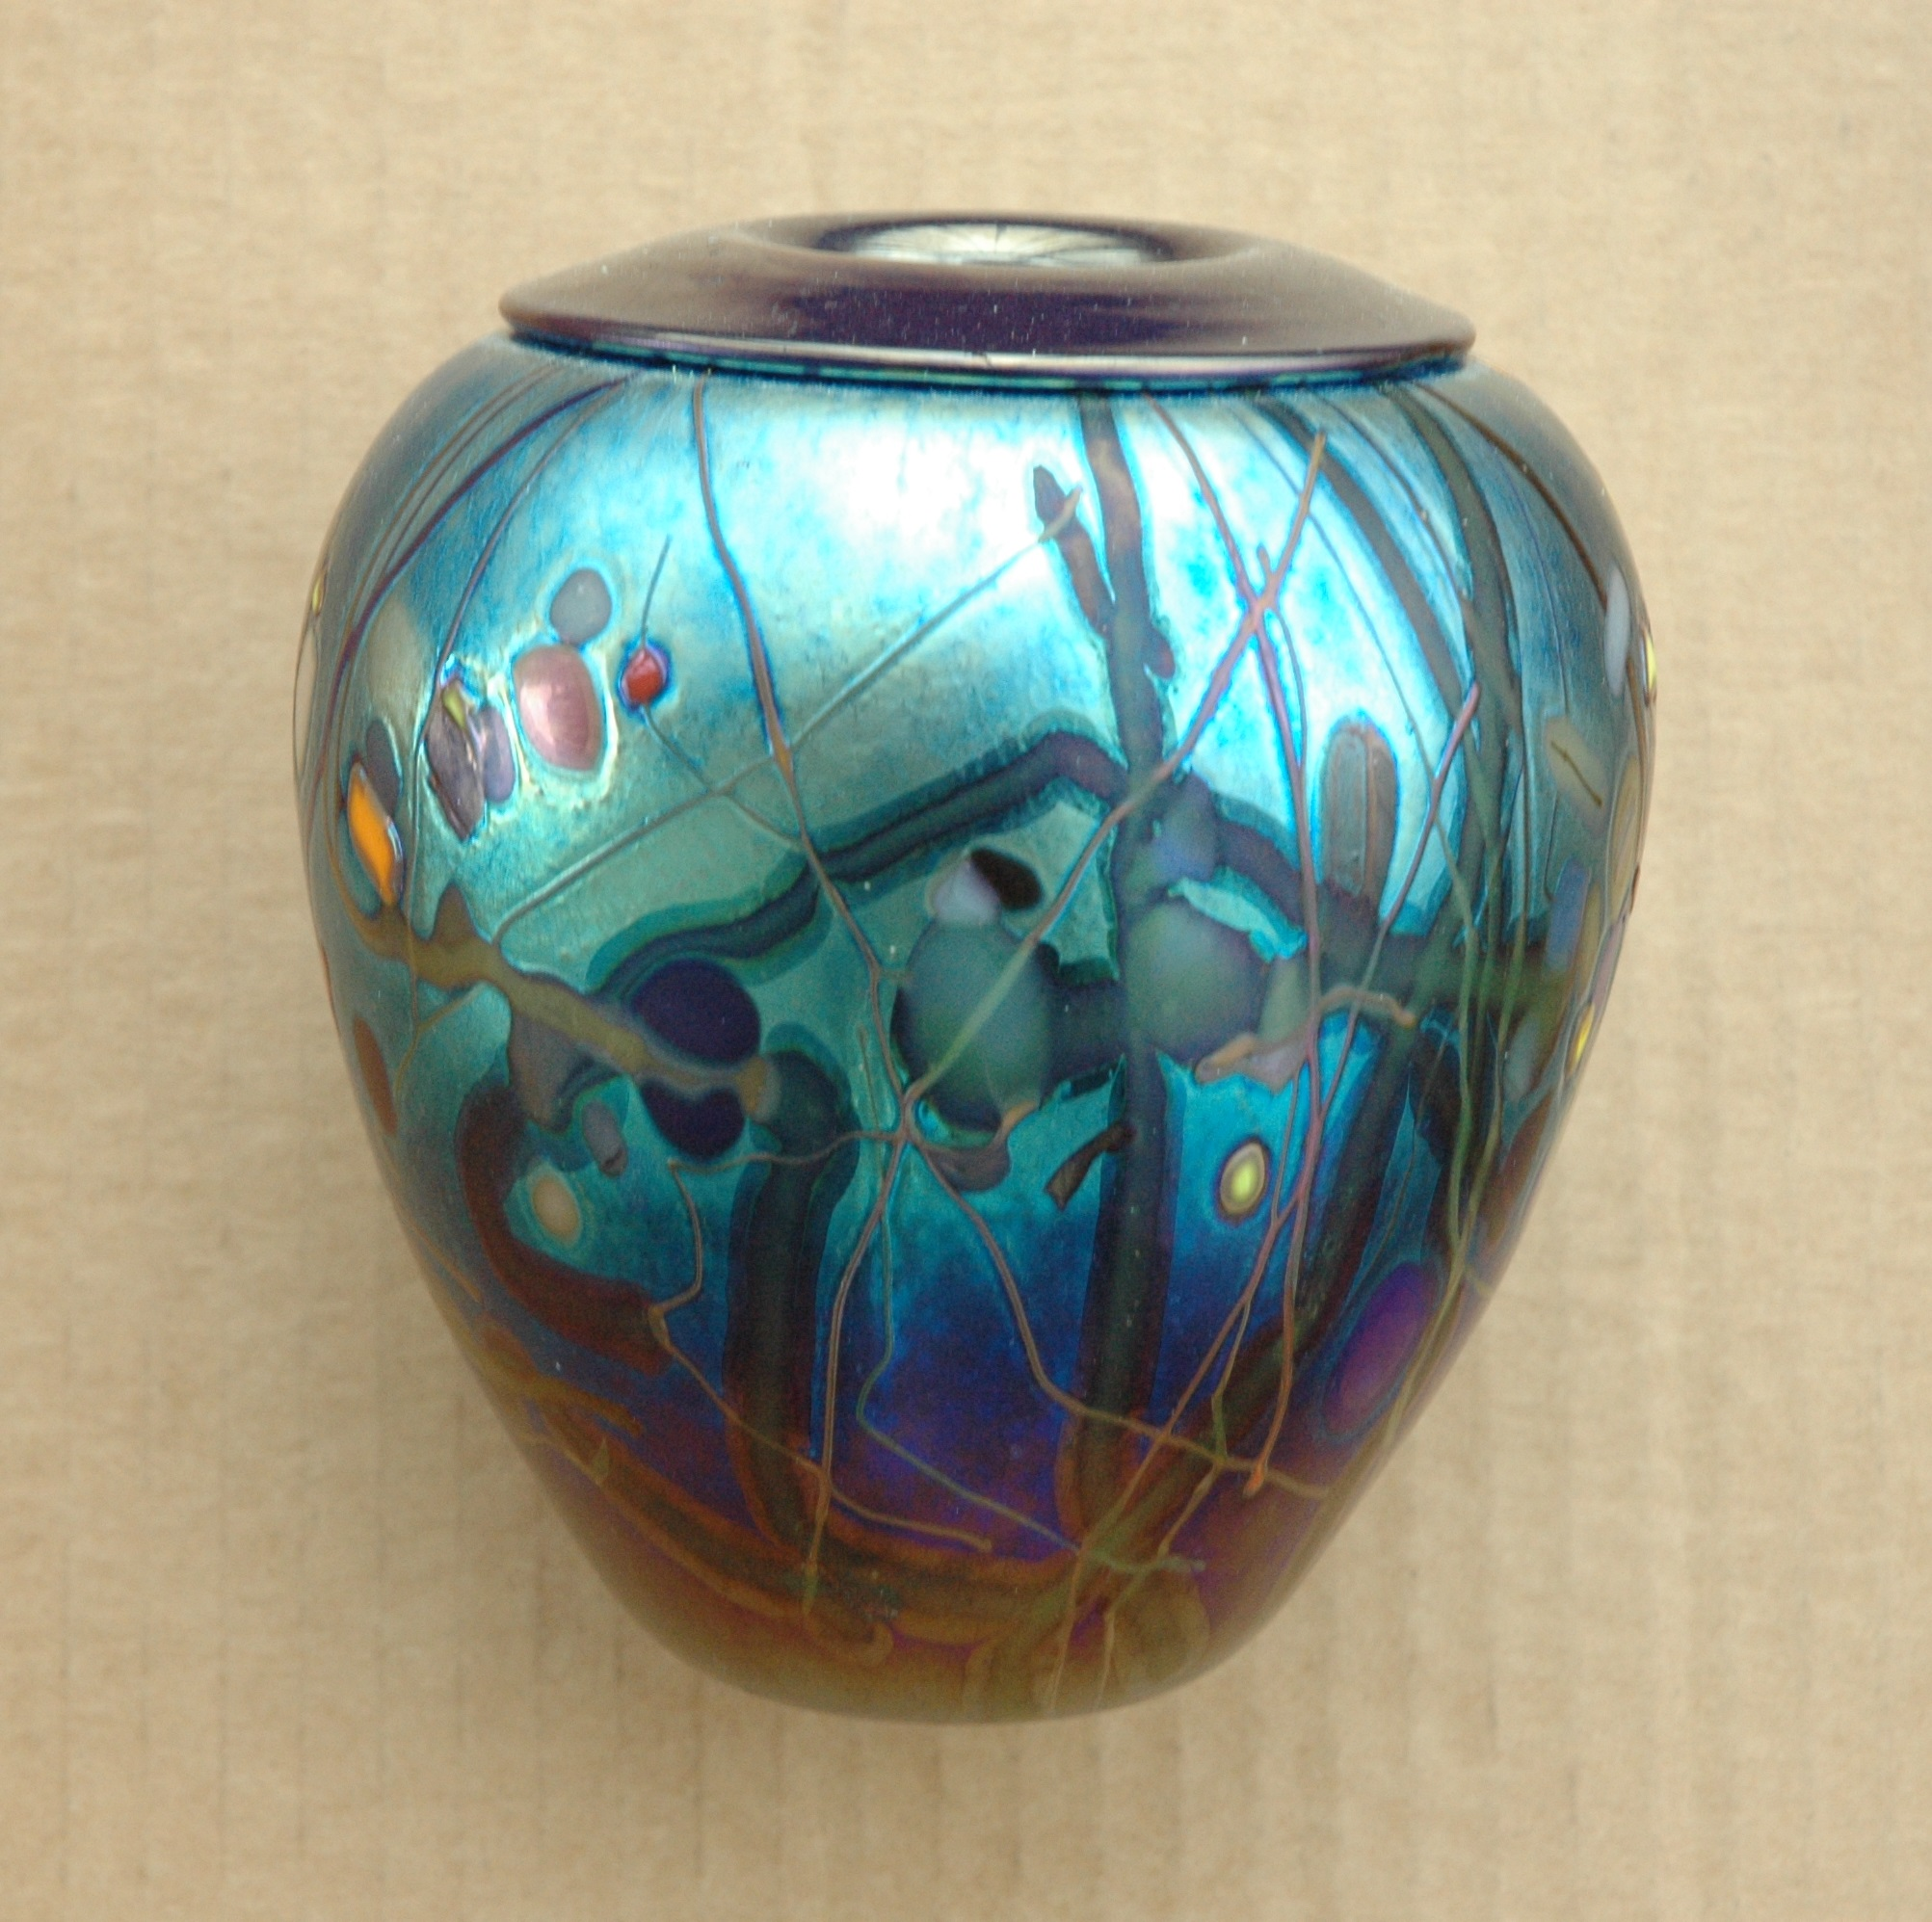
\includegraphics[width=0.33\textwidth]{interp/real_world_img/vase/vase}}\\
  % \includegraphics[width=0.1\textwidth]{interp/real_world_img/pot/base_00} &
  % \includegraphics[width=0.1\textwidth]{interp/real_world_img/pot/base_01} & &
  % \includegraphics[width=0.1\textwidth]{interp/real_world_img/statue/base_00} & & &
  % \includegraphics[width=0.1\textwidth]{interp/real_world_img/vase/base_00} &
  % \includegraphics[width=0.1\textwidth]{interp/real_world_img/vase/base_01}\\
  \multicolumn{3}{c}{(g). pot} & \multicolumn{3}{c}{(h). statue} & \multicolumn{3}{c}{(i). vase} \\
  \end{tabular}
  \caption{Images of the real-world objects.}
  \label{fig:real_data_material}
\end{table}

\section{Parameters of real-world objects}
\begin{table}[!htbp]
  \centering
  \begin{tabular}{*{3}{p{8mm}}*{2}{p{15mm}}|r}
  \toprule
  % & & & & & \multicolumn{3}{c}{Metrics}\\
  Class & Texture & Albedo & Specularity & Roughness & Mapping\\
  \midrule
  box & 0.8 & 0.8 & 0.2 & 0.8 & PMVS, EPS, GSL\\
  cat0 & 0.5 & 0.5 & 0.2 & 0.2 & PMVS\\
  cat1 & 0.2 & 0.2 & 0.2 & 0.2 & None\\
  cup & 0.2 & 0.8 & 0.5 & 0.2 & EPS, GSL\\
  dino & 0.2 & 0.5, 0.8 & 0.2 & 0.8 & EPS, GSL\\
  house & 0.8 & 0.2, 0.8 & 0.2 & 0.2 & PMVS, GSL\\
  pot & 0.8 & 0.2, 0.5 & 0.2 & 0.2 & PMVS\\
  status & 0.2 & 0.8 & 0.2 & 0.8 & EPS, GSL\\
  vase & 0.8 & 0.2, 0.5 & 0.5 & 0.2 & PMVS\\
  \bottomrule
  \end{tabular}
  \caption{Property list for the real-world objects}
  \label{tab:real_data_prop_list}
\end{table}

\section{Results of real-world objects}
\begin{figure}[!htbp]
\centering
\begin{tabular}{l|cccc}
Mapping & PMVS & EPS & GSL & VH (BL)\\
\midrule
PMVS, EPS, GSL &
\fcolorbox{green}{white}{\raisebox{-.5\height}{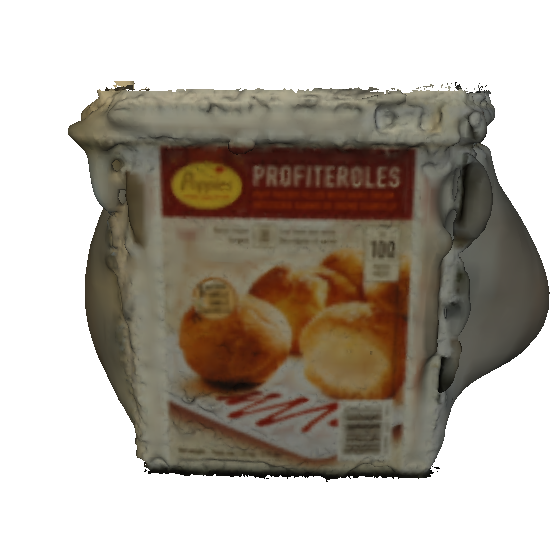
\includegraphics[width=0.2\textwidth]{interp/real_interp/box/box_mvs}}}&
\fcolorbox{green}{white}{\raisebox{-.5\height}{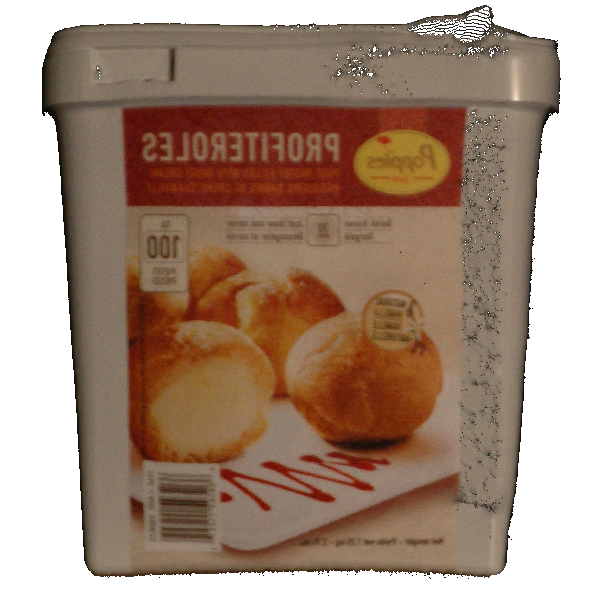
\includegraphics[width=0.2\textwidth]{interp/real_interp/box/box_ps}}}&
\fcolorbox{green}{white}{\raisebox{-.5\height}{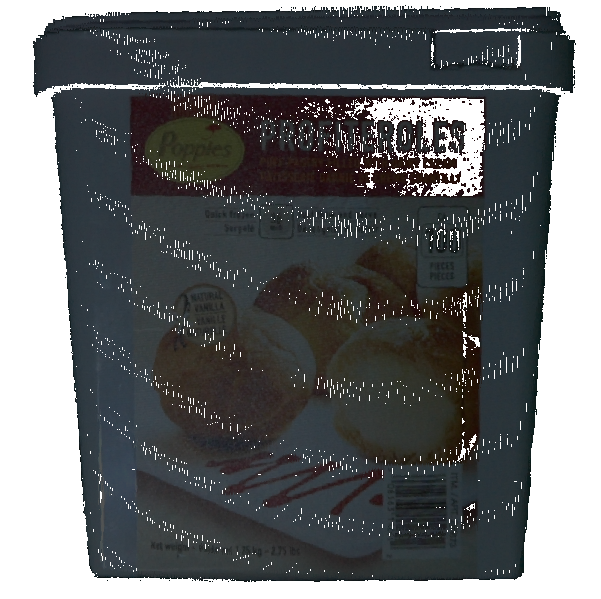
\includegraphics[width=0.2\textwidth]{interp/real_interp/box/box_sl}}}&
\raisebox{-.5\height}{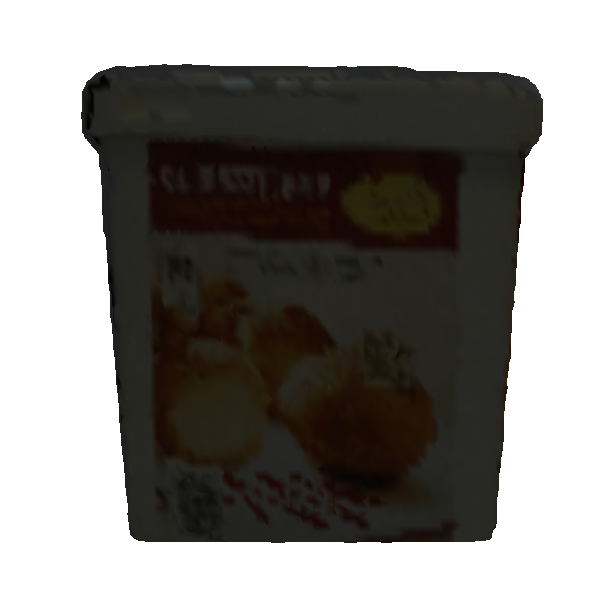
\includegraphics[width=0.2\textwidth]{interp/real_interp/box/box_sc}}\\
PMVS &
\fcolorbox{green}{white}{\raisebox{-.5\height}{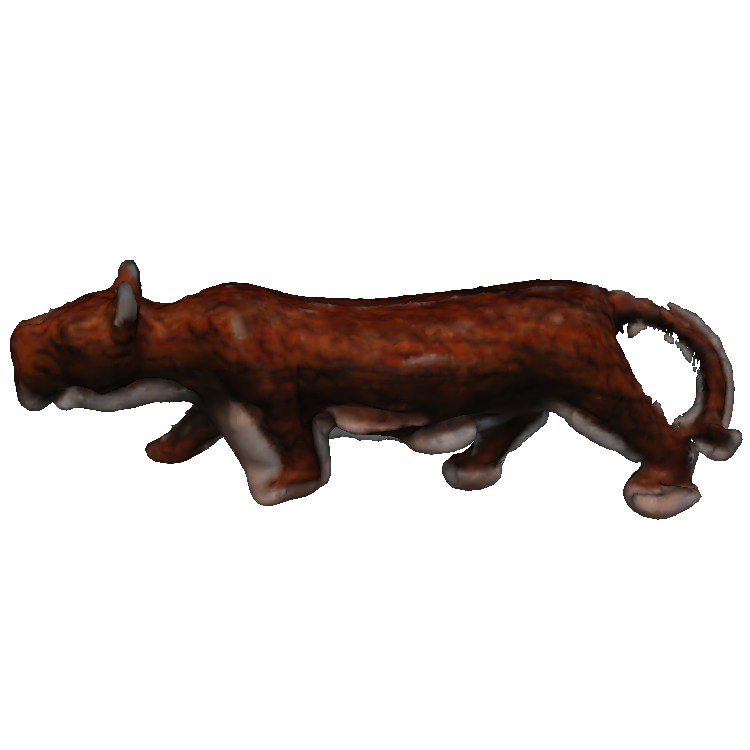
\includegraphics[width=0.2\textwidth]{interp/real_interp/cat0/cat0_mvs}}}&
\raisebox{-.5\height}{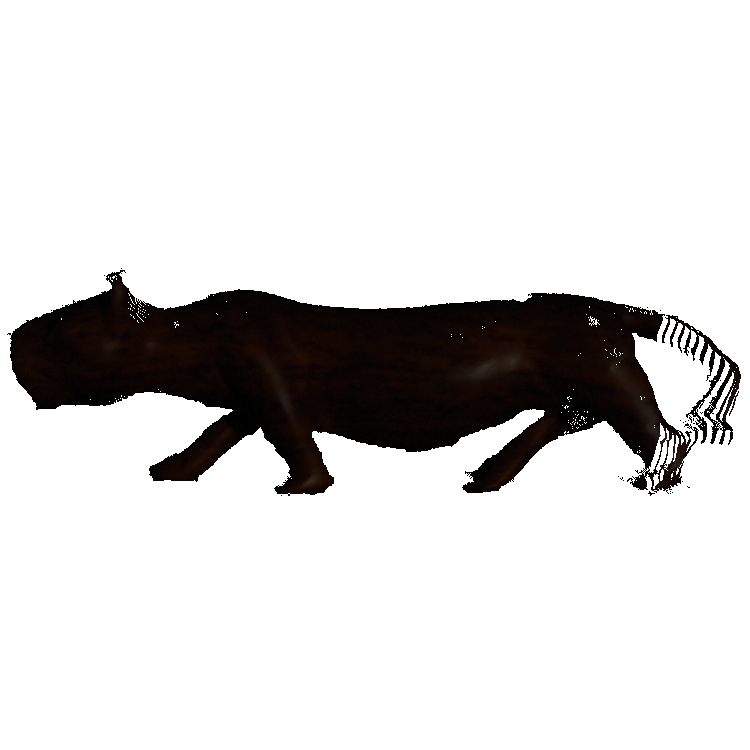
\includegraphics[width=0.2\textwidth]{interp/real_interp/cat0/cat0_ps}}&
\raisebox{-.5\height}{
\includegraphics[width=0.2\textwidth]{interp/real_interp/cat0/cat0_sl}}&
\raisebox{-.5\height}{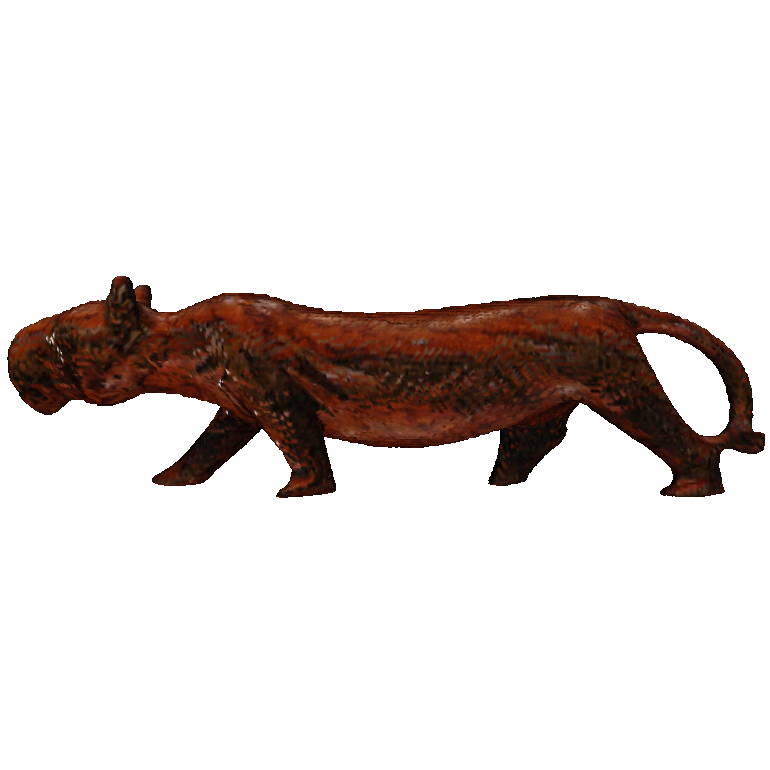
\includegraphics[width=0.2\textwidth]{interp/real_interp/cat0/cat0_sc}}\\
None &
\raisebox{-.5\height}{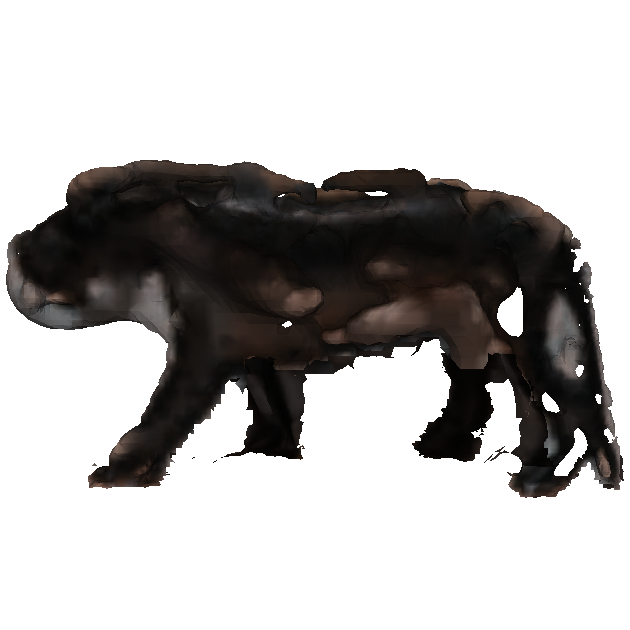
\includegraphics[width=0.2\textwidth]{interp/real_interp/cat1/cat1_mvs}}&
\raisebox{-.5\height}{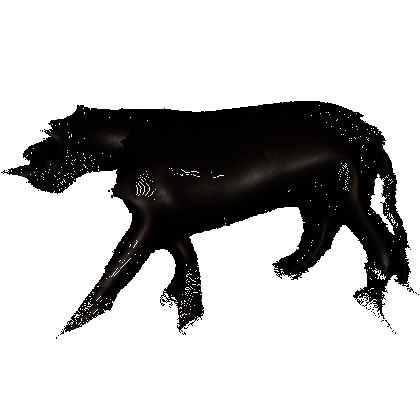
\includegraphics[width=0.2\textwidth]{interp/real_interp/cat1/cat1_ps}}&
\raisebox{-.5\height}{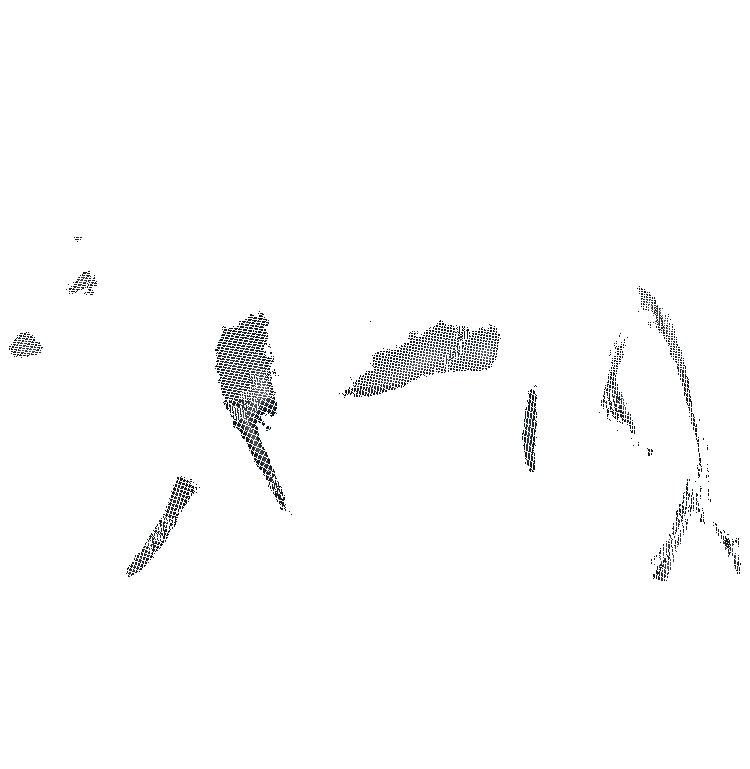
\includegraphics[width=0.2\textwidth]{interp/real_interp/cat1/cat1_sl}}&
\raisebox{-.5\height}{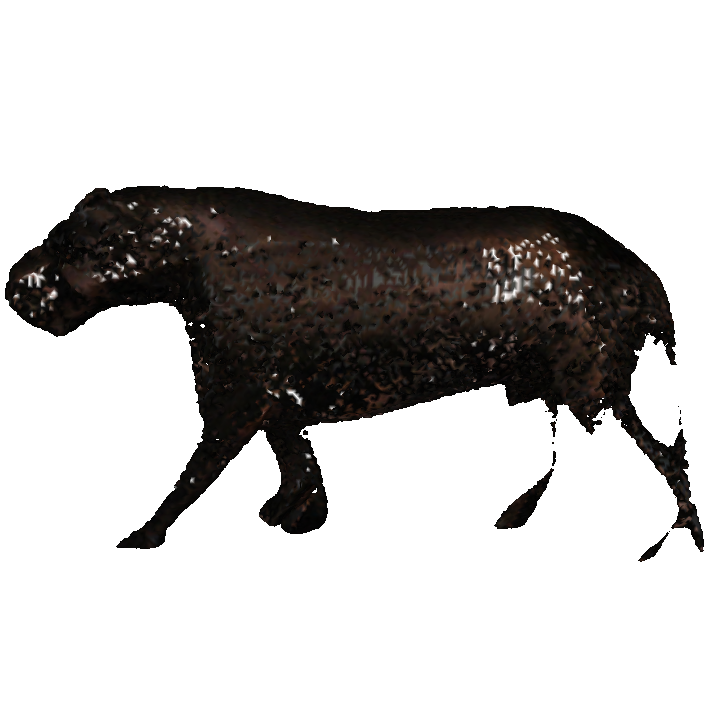
\includegraphics[width=0.2\textwidth]{interp/real_interp/cat1/cat1_sc}}\\
EPS, GSL &
\raisebox{-.5\height}{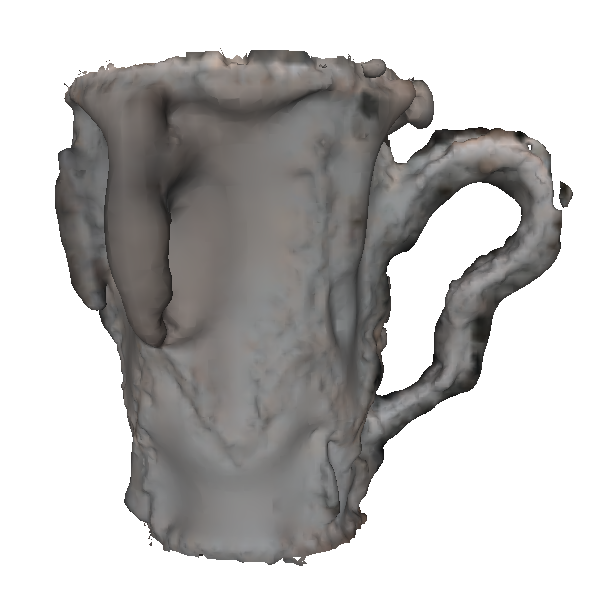
\includegraphics[width=0.2\textwidth]{interp/real_interp/cup/cup_mvs}}&
\fcolorbox{green}{white}{\raisebox{-.5\height}{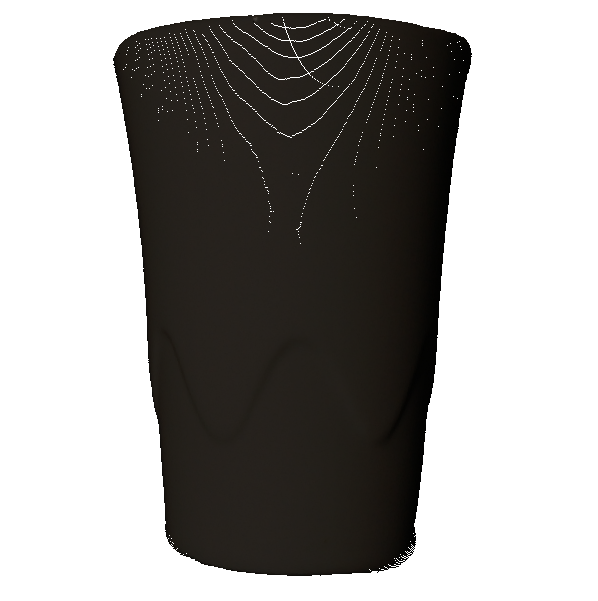
\includegraphics[width=0.2\textwidth]{interp/real_interp/cup/cup_ps}}}&
\fcolorbox{green}{white}{\raisebox{-.5\height}{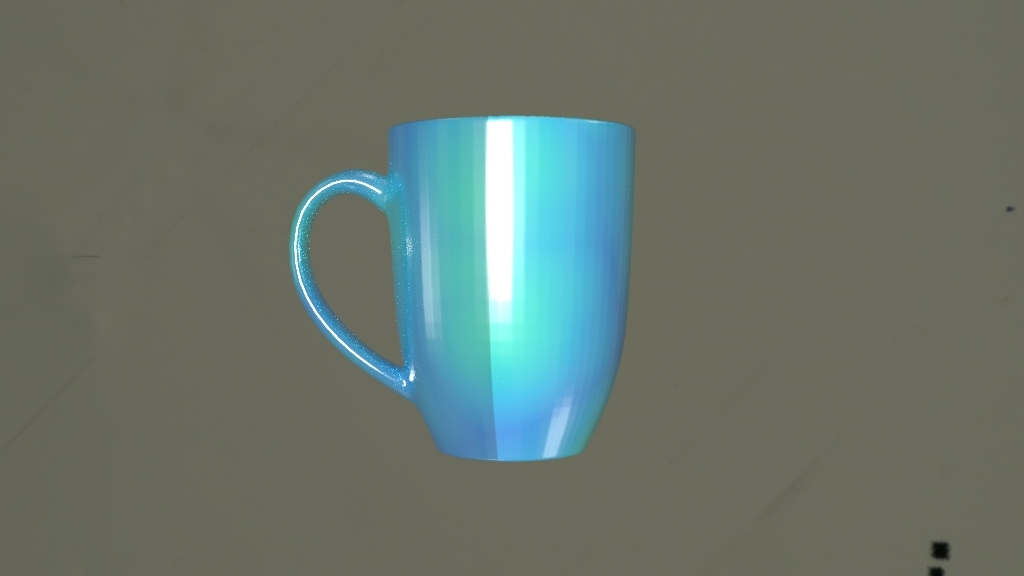
\includegraphics[width=0.2\textwidth]{interp/real_interp/cup/cup_sl}}}&
\raisebox{-.5\height}{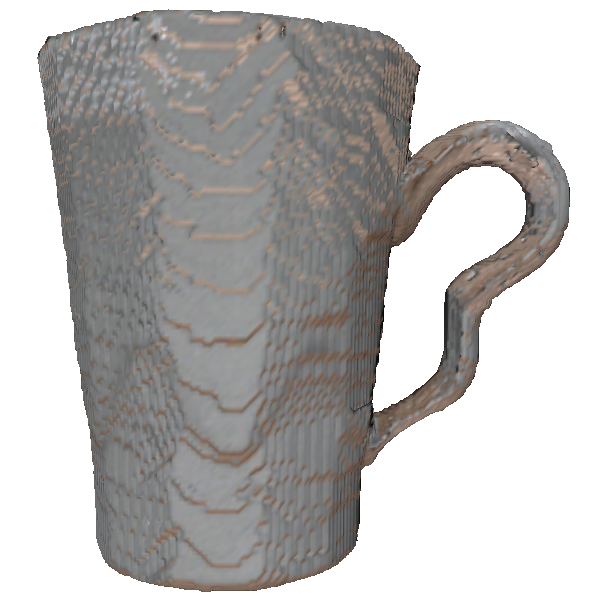
\includegraphics[width=0.2\textwidth]{interp/real_interp/cup/cup_sc}}\\
EPS, GSL &
\raisebox{-.5\height}{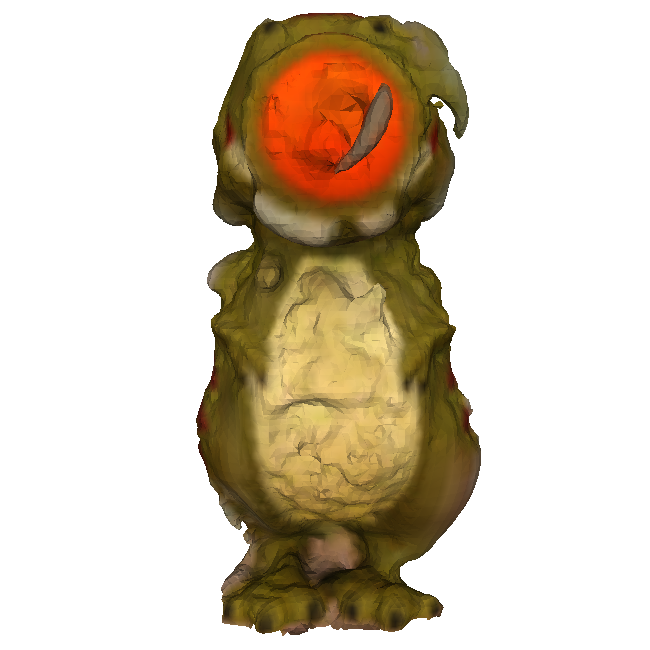
\includegraphics[width=0.2\textwidth]{interp/real_interp/dino/dino_mvs}}&
\fcolorbox{green}{white}{\raisebox{-.5\height}{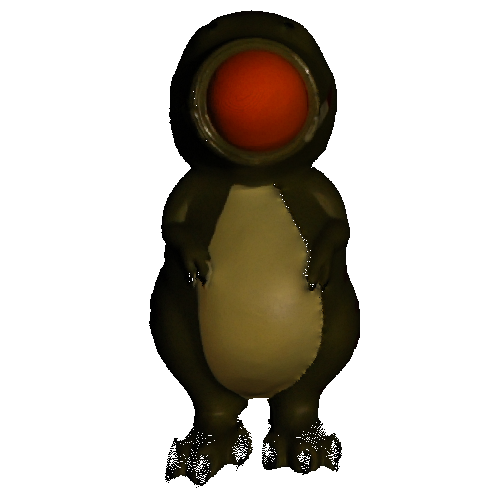
\includegraphics[width=0.2\textwidth]{interp/real_interp/dino/dino_ps}}}&
\fcolorbox{green}{white}{\raisebox{-.5\height}{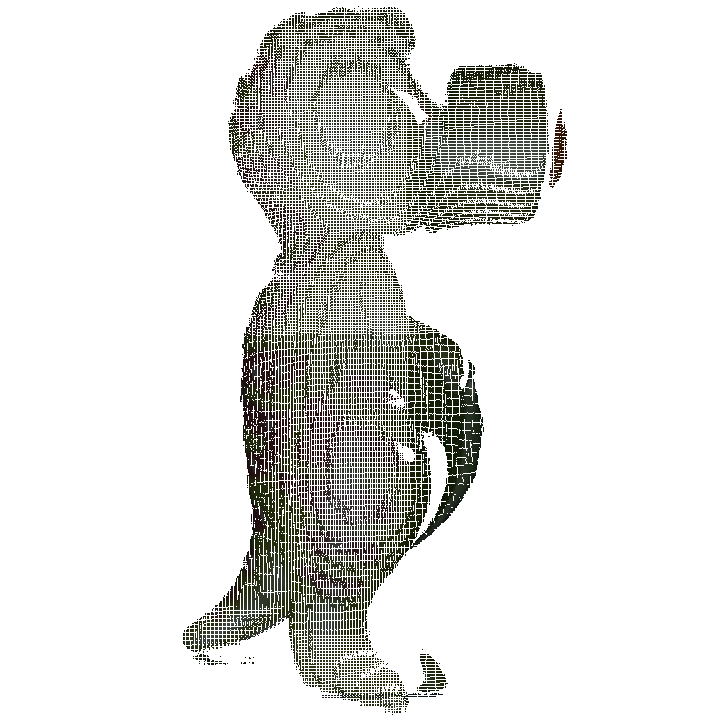
\includegraphics[width=0.2\textwidth]{interp/real_interp/dino/dino_sl}}}&
\raisebox{-.5\height}{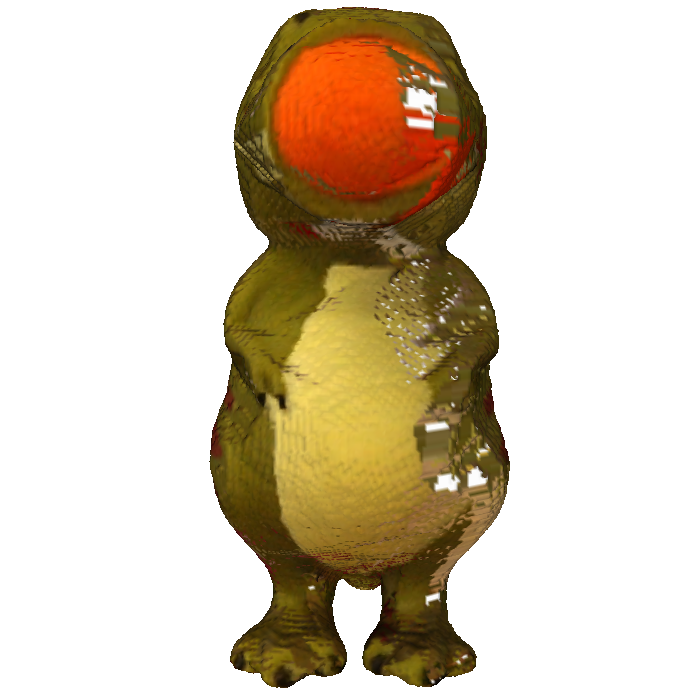
\includegraphics[width=0.2\textwidth]{interp/real_interp/dino/dino_sc}}\\
PMVS, GSL &
\fcolorbox{green}{white}{\raisebox{-.5\height}{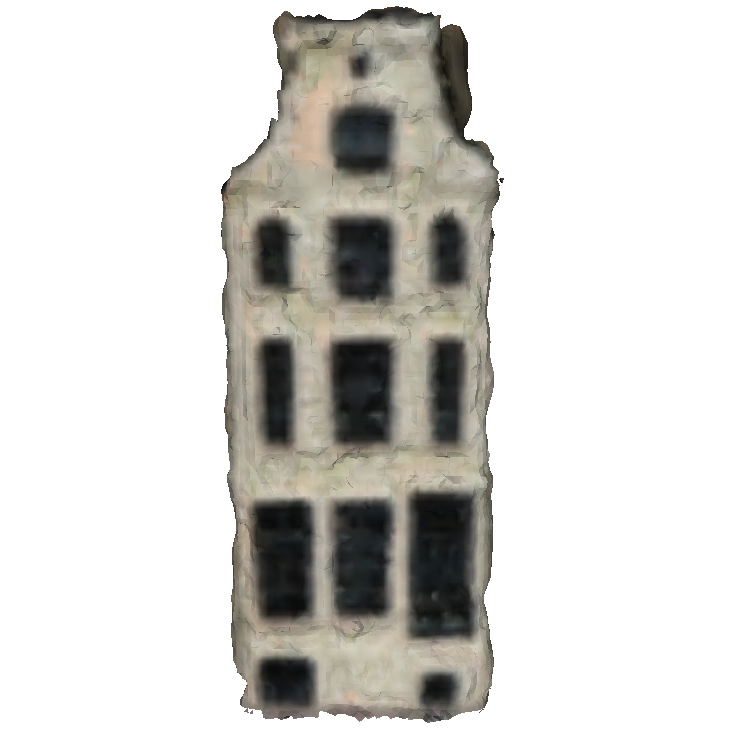
\includegraphics[width=0.2\textwidth]{interp/real_interp/house/house_mvs}}}&
\raisebox{-.5\height}{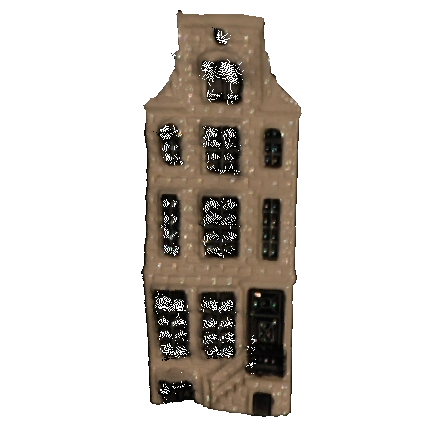
\includegraphics[width=0.2\textwidth]{interp/real_interp/house/house_ps}}&
\fcolorbox{green}{white}{\raisebox{-.5\height}{\includegraphics[width=0.2\textwidth]{interp/real_interp/house/house_sl}}}&
\raisebox{-.5\height}{\includegraphics[width=0.2\textwidth]{interp/real_interp/house/house_sc}}\\
\bottomrule
\end{tabular}
\caption{Reconstruction results of MVS, PS, SL, and the baseline method VH.}
\label{fig:test_real_world_img}
\end{figure}

\begin{figure}[h!]
\centering
\begin{tabular}{l|cccc}
Mapping & PMVS & Example-based PS & Gray SL & VH(BL)\\
\midrule
PMVS &
\fcolorbox{green}{white}{\raisebox{-.5\height}{\includegraphics[width=0.2\textwidth]{interp/real_interp/pot/pot_mvs}}}&
\raisebox{-.5\height}{\includegraphics[width=0.2\textwidth]{interp/real_interp/pot/pot_ps}}&
\raisebox{-.5\height}{\includegraphics[width=0.2\textwidth]{interp/real_interp/pot/pot_sl}}&
\raisebox{-.5\height}{\includegraphics[width=0.2\textwidth]{interp/real_interp/pot/pot_sc}}\\
EPS, GSL &
\raisebox{-.5\height}{\includegraphics[width=0.2\textwidth]{interp/real_interp/statue/statue_mvs}}&
\fcolorbox{green}{white}{\raisebox{-.5\height}{\includegraphics[width=0.2\textwidth]{interp/real_interp/statue/statue_ps}}}&
\fcolorbox{green}{white}{\raisebox{-.5\height}{\includegraphics[width=0.2\textwidth]{interp/real_interp/statue/statue_sl}}}&
\raisebox{-.5\height}{\includegraphics[width=0.2\textwidth]{interp/real_interp/statue/statue_sc}}\\
PMVS &
\fcolorbox{green}{white}{\raisebox{-.5\height}{\includegraphics[width=0.2\textwidth]{interp/real_interp/vase/vase_mvs}}}&
\raisebox{-.5\height}{\includegraphics[width=0.2\textwidth]{interp/real_interp/vase/vase_ps}}&
\raisebox{-.5\height}{\includegraphics[width=0.2\textwidth]{interp/real_interp/vase/vase_sl}}&
\raisebox{-.5\height}{\includegraphics[width=0.2\textwidth]{interp/real_interp/vase/vase_sc}}\\
\bottomrule
\end{tabular}
\caption{Reconstruction results of MVS, PS, SL, and the baseline method VH (cont'd).}
\label{fig:test_real_world_img}
\end{figure}